% Master's thesis — Aaron Bendor — Imperial College London
% Design Engineering Master's Project (MEng)
% Build: pdflatex -> bibtex -> pdflatex -> pdflatex
% (VS Code LaTeX Workshop uses this recipe automatically.)

\documentclass[11pt,a4paper]{article}

% ----------------- Page geometry & typography ---------------------------------
\usepackage[a4paper, margin=1in]{geometry}
\usepackage{setspace}
\setstretch{1.1}
\usepackage{microtype}
\usepackage{lmodern}
\usepackage[T1]{fontenc}
\usepackage[utf8]{inputenc}
\usepackage{titlesec}

% ----------------- Math & symbols ---------------------------------------------
\usepackage{amsmath,amssymb,amsthm,bm}
\usepackage{mathtools}

% ----------------- Algorithm boxes & TikZ schematics --------------------------
\usepackage{algorithm}
\usepackage{algpseudocode}
\usepackage{tikz}
\usetikzlibrary{arrows.meta, positioning, shapes.geometric, fit}

% ----------------- Tables, figures, lists -------------------------------------
\usepackage{booktabs}
\usepackage{array}
\usepackage{graphicx}
\graphicspath{{figures/}}
\usepackage{float}
\usepackage{caption}
\captionsetup{font=small,labelfont=bf}
\usepackage{subcaption}
\usepackage{enumitem}
\setlist{nosep}

% ----------------- Code & verbatim --------------------------------------------
\usepackage{listings}
\usepackage{xcolor}
\definecolor{kw}{HTML}{2255AA}
\definecolor{cm}{HTML}{6E6E6E}
\definecolor{st}{HTML}{007733}
\lstset{
  basicstyle=\ttfamily\footnotesize,
  keywordstyle=\color{kw}\bfseries,
  commentstyle=\color{cm}\itshape,
  stringstyle=\color{st},
  breaklines=true, frame=single, numbers=none,
  showstringspaces=false,
}

% ----------------- Cross-refs & hyperlinks ------------------------------------
\usepackage[hidelinks,colorlinks=false]{hyperref}
\usepackage{cleveref}

% ----------------- Bibliography -----------------------------------------------
% IEEEtran numeric style (matches the example thesis convention).
\usepackage[numbers,sort&compress]{natbib}
\bibliographystyle{IEEEtran}

% ----------------- Section spacing --------------------------------------------
\titlespacing*{\section}{0pt}{2ex}{1ex}
\titlespacing*{\subsection}{0pt}{1.5ex}{0.6ex}
\titlespacing*{\subsubsection}{0pt}{1.2ex}{0.4ex}

% ----------------- Custom macros ----------------------------------------------
\newcommand{\Xo}{X_{\!o}}      % observed-state subset
\newcommand{\pT}{p_{\!T}}      % transition kernel
\newcommand{\pI}{p_{\!I}}      % initial / teleport distribution
\newcommand{\Pchain}{P_{\!T}}  % matrix form
\newcommand{\fobs}{f}          % observed stationary count
\newcommand{\gobs}{g}          % observed hitting-rate matrix
\newcommand{\Lam}{\Lambda}     % log-likelihood-ratio score
\newcommand{\RMAE}{\mathrm{RMAE}}
\newcommand{\AUC}{\mathrm{AUC}}
\newcommand{\KL}{\mathrm{KL}}
\newcommand{\code}[1]{\texttt{#1}}

% ----------------- Title block ------------------------------------------------
\title{\bfseries
  Detection of Externally-Influenced Routing\\
  via Inverse Markov-Chain Methods
}
\author{
  Aaron Bendor\\
  \texttt{aaron.bendor22@imperial.ac.uk}
  \and
  Imperial College London\\
  MEng Design Engineering --- Master's Project
}
\date{\today}

% ==============================================================================
\begin{document}
% ==============================================================================

\maketitle
\thispagestyle{empty}

\begin{abstract}
\noindent Satellite-navigation systems and live traffic services reroute their users around congestion, so observed urban traffic increasingly reflects a mixture of drivers' intrinsic route preferences and externally-influenced routing. This matters because demand estimation, route-choice inference, congestion pricing, and infrastructure-investment decisions all rest on the assumption that observed traffic reveals what drivers actually prefer; when a significant share of trips is steered by an external recommender that itself reacts to congestion, that assumption breaks, and any downstream policy or modelling decision built on it is systematically biased. A practical tool that can distinguish externally-influenced trips from intrinsic ones, even approximately, is therefore a prerequisite for trustworthy inference on modern urban data.

This dissertation designs, validates, and stress-tests a \emph{partial-observation routing-influence filter}: a pipeline that takes a road graph, a small number of observation stations, and two snapshots of traffic taken under different conditions, fits a route-choice model to each snapshot, and scores individual trips by how likely each one is under one model versus the other. The filter is built for partial observation because urban networks contain thousands of road segments while real sensing infrastructure (loop detectors, automatic-vehicle-identification gantries, fixed cameras) typically covers only a few percent of them; any deployable tool must therefore infer behaviour over the whole network from counts at a sparse subset of locations. The inverse-Markov-chain method of Morimura, Osogami and Id\'e~\cite{morimura2013} is the route-choice estimator inside the filter, chosen because it was specifically formulated to recover a chain from such partial observations.

Existing route-choice and demand-estimation methods, from discrete-choice and recursive-logit models to inverse-reinforcement-learning approaches, are formulated for a single homogeneous behavioural regime and require either full trajectory data or strong assumptions about how to fill in unobserved segments. None of them provide a trip-level mechanism for distinguishing intrinsic routing from externally-influenced routing under sparse observation. The novel contribution of this work is to combine a partial-observation inverse-chain estimator with a trip-level log-likelihood-ratio scoring rule and a diagnostic suite that separates genuine route-choice recovery from misleading aggregate effects, producing a complete two-regime filter rather than a single-chain estimator. Three experimental settings justify and audit the design: a synthetic reproduction of the original benchmark, a controlled traffic-simulator study (SUMO~\cite{lopez2018}) in which sat-navigation rerouting is turned on and off for an identical population of vehicles, and a real-world dataset of about 10.5 million reconstructed vehicle trips from Xuancheng, China~\cite{ma2026xuancheng} using rush-hour versus off-peak travel as a behavioural stand-in for sat-navigation use. A second filter variant adds road-network attributes (road class, speed limit, lane count, turn geometry) as shared regularising priors.

The simulator study shows that the filter works end-to-end when ground-truth labels exist: the trip-level score reaches an area under the ROC curve of $0.708$ on a long-trajectory test, against a best-possible value of $0.801$ for any model of this class on the same data. The feature-regularised variant robustly improves how closely the fitted route-choice changes match the true ones at junctions, with the improvement holding across all five repeat simulations tested. A regularised two-step empirical memory test --- interpolation backoff toward the one-step reference, with count-conditional trust on the two-step counts --- lifts the empirical AUC by $+0.10$ on average across five repeat simulations (all five winning), identifying higher-order routing memory as a real design lever and motivating a parametric two-step extension to the inverter as a justified future direction; the optional hitting-rate input of the original method, by contrast, is fully tractable at a sub-network scale where its empirical estimate is informative --- where it lifts AUC by $+0.055$ at an appropriately re-tuned loss weighting and matches the full-observation reference within sampling noise --- but does not naively scale to a full city network because the wide gradient solve in the hitting-rate Jacobian benefits from dense BLAS3 kernels rather than the sparse-LU rewrite the obvious engineering fix would suggest. A simulator decomposition of the rush-hour-vs-off-peak behavioural proxy used on real-world data --- varying sat-navigation adoption and congestion level independently across five repeats --- attributes approximately $96\%$ of the peak-vs-off-peak routing-distribution signal to sat-navigation adoption rather than to congestion-induced rerouting of unaided drivers, supporting the proxy's interpretation in the controlled regime. On the real-world dataset, the filter's diagnostic suite correctly reports a negative result: once population differences between rush-hour and off-peak drivers are controlled, the filter cannot tell the two groups apart at any spatial resolution we tested, even though a full-observation reference weakly can. The contribution is therefore a designed and audited filter, together with a clear account of where it can be trusted (controlled simulation with labels) and where it currently cannot (real-world data without ground-truth labels for who is following a sat-nav).
\end{abstract}


\newpage
\tableofcontents

\newpage
\section{Notation}\label{sec:notation}

A consolidated reference for the mathematical objects used throughout this
report. Notation follows \citet{morimura2013} where it does, and is extended
in \cref{sec:methodology} where required.

\begin{table}[H]
\centering
\caption{Key symbols.}
\label{tab:notation}
\small
\begin{tabular}{@{}lp{0.74\linewidth}@{}}
\toprule
\textbf{Symbol} & \textbf{Meaning} \\
\midrule
$\mathcal{X}$, $n$ & Full state space (directed road edges); $n = |\mathcal{X}|$. \\
$\Xo \subset \mathcal{X}$ & Subset of \emph{observed} states at which counts are available. \\
$\mathrm{adj}(x)$ & Set of legal successors of state $x$ (out-neighbours in the directed graph). \\
$\pT(x'\mid x)$ & One-step transition probability from $x$ to $x'$; row $x$ of the kernel $\Pchain$. \\
$\pI(x)$ & Initial / teleport probability on $\mathcal{X}$; row vector. \\
$\beta \in [0,1]$ & Continuation probability per step; together with $\pI$ defines the stationary mixture $P = \beta\Pchain + (1-\beta)\,\bm{1}\pI^\top$. \\
$\pi$ & Stationary distribution of $P$; obtained from $\pi^\top P = \pi^\top$, $\bm{1}^\top\pi = 1$. \\
$\fobs(x)$ & Empirical visit count (or normalised frequency) at $x$. Observed only for $x \in \Xo$. \\
$\gobs(x, x')$ & Empirical (or analytical) \emph{hitting rate} from $x$ to $x'$, a discounted first-passage probability on $\Xo \times \Xo$. \\
$\phi_T(x') \in \mathbb{R}^{d_T}$ & Destination-state feature vector (\cref{sec:features}). \\
$\psi(x, x') \in \mathbb{R}^{d_\psi}$ & Directed-edge feature vector. \\
$\nu \in \mathbb{R}^n$ & Per-state base parameters of $\pI$. \\
$\omega^{\mathrm{loc}} \in \mathbb{R}^E$ & Per-edge local weights of $\pT$, with $E = \sum_x |\mathrm{adj}(x)|$ the number of directed edges. \\
$\omega^{\mathrm{glo}_1} \in \mathbb{R}^{d_T}$ & Shared weights on destination features $\phi_T$ (paper Eq.~17). \\
$\omega^{\mathrm{glo}_2} \in \mathbb{R}^{d_\psi}$ & Shared weights on edge features $\psi$ (paper Eq.~17). \\
$\theta$ & Full parameter vector $[\nu;\omega^{\mathrm{loc}};\omega^{\mathrm{glo}_1};\omega^{\mathrm{glo}_2}] \in \mathbb{R}^{d}$, $d = n + E + d_T + d_\psi$. \\
$\lambda$ & Tikhonov regularisation strength on $\|\theta\|^2$. \\
$\gamma \in [0,1]$ & Mixing weight between the stationary-match loss $L_d$ and the hitting-rate loss $L_h$. \\
$\Lam(\tau)$ & Log-likelihood-ratio score of a test trajectory $\tau$ under two fitted chains (\cref{sec:methodology}). \\
$\AUC$ & Area under the ROC curve of the LR score against labelled regime test trajectories. \\
$\RMAE(\hat{\pi},\pi)$ & Relative mean absolute error of recovered stationary mass at unobserved states. \\
\bottomrule
\end{tabular}
\end{table}

Throughout, ``regime'' refers to one of two distinguishable driver
populations whose chains we fit and compare. In controlled simulation
this is intrinsic vs.\ sat-navigation-influenced; in real-world data it
is a behavioural proxy (e.g.\ rush-hour vs.\ off-peak). The contrast
$\Delta_{\mathrm{fit}}(x, \cdot) = \pT^{(B)}(x,\cdot) - \pT^{(A)}(x,\cdot)$
between two fitted chains is the central quantity assessed against the
empirical ground-truth contrast
$\Delta_{\mathrm{emp}}(x, \cdot)$.


\section{Introduction}\label{sec:introduction}

\subsection{Context: urban traffic and the external-influence problem}
\label{sec:context}

The widespread adoption of satellite-navigation applications such as Google
Maps, Waze, and TomTom has structurally altered how vehicles use urban road
networks. These systems no longer merely report a single shortest path:
they reroute users in real time around observed congestion, redistributing
traffic across alternative arteries on time-scales of minutes to hours.
The consequence is that any traffic observation aggregating across modern
drivers reflects a \emph{mixture} of two distinct routing rules: the
intrinsic preferences a driver would express in the absence of guidance
(habit, scenic preference, fuel-cost optimisation, familiarity), and the
external recommendations of a sat-navigation system reacting to live
network state.

This mixture creates a problem for downstream traffic models. Demand
estimation, route-choice inference, transport-policy evaluation, and
infrastructure-investment decisions all rely on revealed-preference data
that is assumed to encode \emph{driver} preferences. When a sizeable
fraction of observed trips are guided by an external recommender that
itself responds to congestion (and thereby to other guided trips), the
revealed data encodes a partially synthetic, congestion-coupled signal
that the underlying driver population would not have produced unaided.
Identifying and filtering this externally-influenced traffic, or at minimum
quantifying its presence, has therefore become a methodological
prerequisite for any inference about driver behaviour in modern urban
environments.

\subsection{Inverse Markov-chain methods and the Morimura framework}
\label{sec:intro-morimura}

A long line of work models route choice as a Markov chain over road
network edges, in which each driver, conditional on their current edge,
selects a next edge with probabilities determined by local and global
features of the network. \citet{morimura2013} introduced an
\emph{inverse} formulation that fits the parameters of such a chain
from only partial observations of the network --- specifically, from
vehicle counts at a small subset of observation stations $\Xo$ and
optionally from pairwise hitting rates between those stations. Their
softmax-parametric chain admits an analytic gradient of the regularised
log-ratio loss, enabling reliable fitting on networks of several
thousand edges with $20\text{--}90\%$ observation coverage.

The Morimura framework is well validated on synthetic data and was
applied by its authors to one real-world traffic case study in Nairobi.
It has not, however, been adapted to the specific problem of detecting
externally-influenced routing as distinct from intrinsic preferences:
the original work treats the inverse problem as one of \emph{recovering}
a single chain, not of \emph{distinguishing} two coexisting routing
regimes within the same network.

\subsection{Contributions}
\label{sec:contributions}

This dissertation extends the Morimura inverse-Markov-chain method into a
three-tier detection pipeline for externally-influenced routing, validates
each tier honestly, and quantifies where the framework's limits actually
lie. Specifically:

\begin{enumerate}
\item \textbf{Faithful synthetic reproduction of the Morimura $\S 6.1$
benchmark.} We re-implement the inverter, derive and
finite-difference-verify the analytic gradients (including the
omega-global gradient extensions for shared destination and edge features
that the paper states but does not derive in full), and reproduce the
proposed-method RMAE curve of Fig.~2A in \cite{morimura2013} closely for
observation fractions $\Xo/n \ge 0.10$. The very-low-observation point
($|\Xo|=5$) and the NWKR comparator are documented deviations
(\cref{sec:phase1-synthetic}). This locks in the upstream implementation
as a faithful operational reference.

\item \textbf{A SUMO regime detector under partial observation with real
edge features.} We construct a bigger-bbox SUMO scenario in which an
identical population of vehicles is simulated twice --- once with no
sat-navigation rerouting (static unguided routing) and once with full
sat-navigation rerouting --- fit a Morimura inverter to each regime's
partial observations, and feed the fitted chains to a per-trajectory
log-likelihood-ratio detector. On the representative seed the detector
reaches $\AUC = 0.644$ at $T=20$ against a full-observation empirical
$1$-step reference of $0.685$, rising to $\AUC = 0.708$ at $T=40$ against
a reference of $0.801$ as the scoring window widens.

\item \textbf{Per-row contrast diagnostics separating chain recovery from
aggregate AUC.} Following the observation that detection AUC can improve
through aggregate chain-drift rather than correct per-row recovery, we
report a contrast-correlation diagnostic at branching states. Real edge
features robustly improve \emph{per-row chain recovery} across a five-seed
sweep (stacked Pearson $+0.050 \pm 0.023$, $p \approx 0.008$, positive on
all five seeds), whereas the aggregate detection-AUC lift is
seed-dependent rather than robust ($+0.024 \pm 0.026$, reversing on one
of five seeds). Features are best described as a chain-recovery lever, not
an aggregate-detection lever.

\item \textbf{An empirical higher-order memory diagnostic.} A natural
hypothesis is that the residual gap is missing $2$-step memory. We test
this with a fitting-free empirical $2$-step detector --- counting
$(x_{t-1}, x_t)\to x_{t+1}$ triples on the same trajectories --- and find
it does \emph{not} improve over the $1$-step empirical reference
($\AUC_{2\text{-step}} = 0.666 < \AUC_{1\text{-step}} = 0.685$). This
weakens the case for implementing a parametric $2$-step extension as the
immediate next step, but does not rule out regularised, feature-based,
destination-aware, or hierarchical higher-order models.

\item \textbf{A real-world stress test with OD-rebalancing on the
Xuancheng AVI dataset.} We port the pipeline to $\sim 10.5$ million
reconstructed vehicle trips over April~2023 \cite{ma2026xuancheng}. Because
no real dataset comes with sat-navigation adoption labels, we use a
time-of-day behavioural proxy (rush-hour vs.\ off-peak) and introduce an
OD-rebalancing step that subsamples each regime to share the same
$(\mathrm{origin\ zone},\mathrm{destination\ zone})$ distribution. This
controls the population-mix confound and shows that most of the apparent
proxy contrast is OD-mix, not routing choice (\cref{sec:phase5-xuancheng}).
A single CLI runs all three tiers via a \code{--dataset \{sumo,xuancheng\}}
flag; the repository structure is documented in \cref{app:repo}.
\end{enumerate}

\subsection{Roadmap}
\label{sec:roadmap}

\cref{sec:background} situates the work in relevant prior literature.
\cref{sec:methodology} presents the mathematical framework and the three
extensions (real features, $2$-step diagnostic, OD-rebalancing) in detail.
\cref{sec:phase1-synthetic,sec:phase4-sumo,sec:phase5-xuancheng}
present the three validation tiers in turn, each one with its own
honest discussion of what does and does not transfer. \cref{sec:discussion}
draws cross-tier conclusions and limitations. \cref{sec:reflection}
addresses project management and personal-development reflection per the
module's \emph{Reflection} learning outcome \cite{markscheme}.


\section{Background and Related Work}\label{sec:background}

\subsection{Inverse problems on Markov chains}
\label{sec:inverse-mc}

A Markov chain is a stochastic process in which the next state depends
only on the current state. The \emph{forward} problem asks, given a
transition kernel $\Pchain$, what statistics (stationary distribution,
hitting times, expected occupation, etc.) does the chain produce? The
\emph{inverse} problem reverses this: given partial statistics observed
on the chain, recover the transition kernel itself. Inverse problems on
Markov chains arise in transport modelling \cite{ben-akiva1985},
biological systems \cite{noe2008}, and recommender systems
\cite{huang2018}, and are typically ill-posed under sparse observation
because many distinct kernels produce identical low-order statistics.
The usual remedy is a parametric restriction: rather than fit
$\Pchain \in \mathbb{R}^{n \times n}$ directly, one fits a parameter
vector $\theta \in \mathbb{R}^d$ with $d \ll n^2$ such that the
parametric form $\Pchain(\theta)$ is constrained to lie in a manifold of
plausible chains. The choice of parametric family is then load-bearing:
the wrong family caps recovery quality regardless of optimisation
effort.

\subsection{Route choice as a softmax-parametric Markov chain}
\label{sec:route-softmax}

In the route-choice setting the state space $\mathcal{X}$ is the set of
directed road edges and the kernel
$\pT(x'\mid x)$ is the probability that a vehicle currently on edge $x$
moves next to edge $x'$. Multinomial-logit route-choice models
\cite{ben-akiva1985, frejinger2007} parametrise the transition
probability as a softmax over the legal successors of $x$:
\begin{equation}
\pT(x'\mid x) \;=\;
\frac{\exp\bigl(s(x, x')\bigr)}{\sum_{x'' \in \mathrm{adj}(x)} \exp\bigl(s(x, x'')\bigr)},
\label{eq:softmax}
\end{equation}
where $s(x, x')$ is a real-valued score, typically a linear combination
of features of the edge $(x, x')$ and of the destination state $x'$.
This formulation has two important properties for inverse problems.
First, it is parameter-efficient: one global feature shared across
many states adds one parameter, regardless of network size. Second, its
gradient is analytic in $s$, which combined with the chain-rule
propagation through stationary computations and hitting-rate solves makes
$\nabla_\theta \log \pi$ and $\nabla_\theta \log \gobs$ tractable to
derive in closed form.

\subsection{The Morimura inverse-MC framework}
\label{sec:morimura}

\citet{morimura2013} apply the softmax form of \cref{eq:softmax} to the
partial-observation regime in which the modeller observes only a
small subset $\Xo \subset \mathcal{X}$. They consider two empirical
observation types:
\begin{itemize}
\item \textbf{Empirical stationary distribution $\fobs$ at $\Xo$.}
A count of vehicle passages at each station; effectively a sample of
$\pi(x)$ for $x \in \Xo$.
\item \textbf{Empirical hitting rates $\gobs(x, x')$ on $\Xo \times \Xo$.}
The fraction of vehicles observed at $x$ that subsequently visit $x'$
discounted by their travel time; effectively a sample of the
$\beta$-discounted first-passage probability.
\end{itemize}
They define a regularised loss that mixes a log-ratio match on $\fobs$
(via the stationary distribution of the parametric chain) and a log-error
match on $\gobs$ (via the hitting-rate matrix of the parametric chain),
weighted by a mixing parameter $\gamma$. Their key contribution is the
analytic derivation of the gradient of this loss with respect to
$\theta$, enabling optimisation via L-BFGS-B or, alternatively, the
natural-gradient descent the paper introduces in $\S 4.1$ as the
optimiser of choice when the loss landscape is ill-conditioned.

The paper validates the framework synthetically on a $n=100$ network
(their $\S 6.1$) and applies it to a $1497$-link Nairobi minibus
network as a real-world demonstration ($\S 6.2$). Both validations report
favourable RMAE on the recovered stationary distribution. Two limitations
of this validation are directly relevant to our work. First, the
synthetic experiment uses analytical (i.e.\ noise-free) hitting rates
$\gobs$ computed from the true chain; on noisy real-world data the
empirical $\gobs$ is overwhelmingly sparse, an effect documented in
\cref{sec:phase4-fg-infeasible}. Second, the real-world Nairobi case is
not framed as a regime-detection problem: the authors do not split the
data into two coexisting routing populations and ask whether the chain
recovery distinguishes them.

\subsection{Re-routing detection and external traffic influence}
\label{sec:rerouting-prior}

Detecting externally-influenced rerouting is a relatively recent
research direction. \citet{gu2018} proposed a junction-level
anomaly-detection approach in which deviations from a learned
turning-distribution baseline serve as evidence of unusual routing
behaviour; their setup is restricted to snapshot-level (population-level)
detection rather than per-trajectory. Active-routing-game analyses
\cite{thai2016, krichene2018} model the equilibrium effects of
sat-navigation adoption on aggregate network performance, but assume a
known navigation rule and focus on welfare bounds rather than detection.
Closest in spirit to this work is the line of route-choice research
that combines partially observed counts with route-fragment
likelihoods \cite{flotterod2017}: this addresses estimation under
partial observation but does not separate populations.

To our knowledge no prior work combines the Morimura inverse-MC
framework with a regime-detection objective, evaluated across both
controlled simulation and real-world data with an OD-mix-controlled
contrast. That is the gap this thesis addresses.

\subsection{Microscopic traffic simulation: SUMO}
\label{sec:sumo}

Simulation of Urban MObility (SUMO) \cite{lopez2018} is the open-source
microscopic traffic simulator used in this thesis to construct the
controlled validation tier (\cref{sec:phase4-sumo}). Each vehicle is
simulated with realistic car-following and lane-change dynamics on a
network derived from OpenStreetMap. Crucially, SUMO exposes a
\code{--device.rerouting.probability} flag that, when set to $1.0$,
gives each vehicle access to an internal congestion-aware
sat-navigation device; when set to $0.0$, vehicles route via static
shortest-path Dijkstra. By running an identical vehicle population
twice with that flag toggled, we obtain a controlled labelled
comparison --- intrinsic-routed vs.\ sat-navigation-routed --- against
which the Morimura-based detector can be honestly benchmarked.

\subsection{Real-world traffic from Automatic Vehicle Identification}
\label{sec:avi-prior}

AVI systems (Automatic License Plate Recognition cameras at selected
junctions, optionally extended with Bluetooth or floating-car-data
fusion) have produced a small but growing collection of openly
released city-scale traffic datasets. Among recent releases:
the Padua AVI deposit \cite{cappi2026} provides $10$-minute aggregated
flow statistics and pairwise travel times over $40$ junctions but
explicitly strips per-vehicle trajectories for privacy; the
Wang \emph{et al.}\ Xuancheng dataset \cite{wang2023xuancheng}
similarly restricts raw trajectory access; the
\citet{ma2026xuancheng} Xuancheng dataset --- used in this thesis ---
releases joinable entry/exit tables with anonymised vehicle IDs from
which complete trajectories can be reconstructed, covering
$\sim 350{,}000$ trips/day across $\sim 1{,}760$ road segments for the
month of April~2023. The Ma~\emph{et al.}\ release is, to our knowledge,
the largest openly available city-scale AVI dataset with
per-vehicle granularity at the time of writing.


\section{Methodology}\label{sec:methodology}

This section presents the inverse Markov-chain framework and the three
extensions developed in this work. \cref{sec:morimura-formulation}
restates the framework in our notation. \cref{sec:features}--\ref{sec:od-rebal}
present the extensions in turn.

\subsection{Parametric chain and observation model}
\label{sec:morimura-formulation}

The state space $\mathcal{X}$ is the set of directed road edges in the
largest strongly-connected component of the network. For each state
$x \in \mathcal{X}$, the next-state distribution is the softmax of
\cref{eq:softmax} over the legal successors $\mathrm{adj}(x)$, with the
score
\begin{equation}
s(x, x') \;=\; \omega^{\mathrm{loc}}_{(x,x')}
\;+\;
\underbrace{\phi_T(x')^\top \omega^{\mathrm{glo}_1}}_{\text{destination-feature term}}
\;+\;
\underbrace{\psi(x, x')^\top \omega^{\mathrm{glo}_2}}_{\text{edge-feature term}}.
\label{eq:score}
\end{equation}
Without the global terms ($d_T = d_\psi = 0$) the model has one
parameter per directed edge; with global terms it adds $d_T + d_\psi$
\emph{shared} parameters that apply across all edges of compatible type.
The initial distribution $\pI$ is similarly parametrised by per-state
weights $\nu \in \mathbb{R}^n$ via $\pI(x) \propto \exp(\nu_x)$.

We define the absorbing-corrected stationary mixture
\begin{equation}
P \;=\; \beta\,\Pchain \;+\; (1-\beta)\,\bm{1}\pI^{\!\top},
\qquad
\pi^{\!\top} P = \pi^{\!\top}, \quad \bm{1}^{\!\top}\pi = 1,
\label{eq:stationary}
\end{equation}
which models the long-run occupancy of a chain that occasionally restarts
from $\pI$ with probability $1-\beta$ per step. The hitting-rate matrix
$H(\Pchain) \in [0,1]^{|\Xo|\times|\Xo|}$ has entries equal to the
$\beta$-discounted first-passage probability between observation states,
obtained as $H_{ij} = [(I - \beta\Pchain^{(\setminus j)})^{-1}]_{ix_j}$
where $\Pchain^{(\setminus j)}$ zeroes row $j$ to encode absorption.
The Morimura observation model says we observe noisy $\fobs(x)$ for
$x \in \Xo$ and noisy $\gobs(x, x')$ for $(x, x') \in \Xo \times \Xo$,
and we wish to match the model's $\pi$ and $H$ to these observations.

\subsection{Regularised loss and analytic gradients}
\label{sec:loss-gradients}

Following \cite{morimura2013} Eqs.~7--9, the loss is the sum of a
stationary-match term, a hitting-rate-match term, and a Tikhonov ridge:
\begin{align}
L(\theta) &= \gamma\,L_d(\theta) + (1-\gamma)\,L_h(\theta) + \lambda\,R(\theta), \\
L_d(\theta) &= \tfrac{1}{2}\sum_{i, j \in \Xo}\bigl(\log\tfrac{\pi_i}{\pi_j} - \log\tfrac{f_i}{f_j}\bigr)^2, \\
L_h(\theta) &= \tfrac{1}{2}\sum_{i, j \in \Xo}\bigl(\log H_{ij} - \log g_{ij}\bigr)^2, \\
R(\theta) &= \tfrac{1}{2}\|\theta\|^2.
\end{align}
Both data terms are log-ratio losses, which is what makes them
optimisable without normalising constants on the observations
\cite{morimura2013}: any multiplicative scale on $\fobs$ or $\gobs$
cancels in the difference. The gradients are derived using the
identity for the derivative of $\log\pi$ under a softmax-parametric
chain (paper Eq.~12) and the derivative of $\log H_{ij}$ under an
absorbing-chain solve (Eq.~15). The paper's local-only gradients
$\partial L / \partial \nu$ and $\partial L / \partial \omega^{\mathrm{loc}}$
are reproduced unchanged here; we derive the omega-global
gradients (paper Eqs.~17--18 \emph{state} the parametric extension but
do not derive the gradients) by writing the chain-rule contribution of
$\omega^{\mathrm{glo}_1}$ and $\omega^{\mathrm{glo}_2}$ through the
score \eqref{eq:score} and chaining through $\nabla_\theta \log \pi$ and
$\nabla_\theta \log H$.

We verify the analytic gradients by centred finite differences
(\code{fd\_check\_features.py}) at random parameter draws across
all four blocks ($\nu$, $\omega^{\mathrm{loc}}$, $\omega^{\mathrm{glo}_1}$,
$\omega^{\mathrm{glo}_2}$). The check uses a noise-aware tolerance
($\code{rtol}=10^{-3}$ relative \emph{or} $\code{atol}=5 \times 10^{-2}$
absolute, an \code{np.allclose}-style criterion) to handle the
machine-precision FD round-off floor that dominates near-zero gradient
components. The bigger-bbox SUMO graph passes at machine precision
($\sim 10^{-8}$ relative error) on the clearly non-zero components.

\subsection{Extension 1: real edge features from the network topology}
\label{sec:features}

The Morimura framework treats $\phi_T$ and $\psi$ as user-supplied global
features. In simulated $\S 6.1$ both are drawn iid
$\mathcal{N}(0,1)$ in their setup; in their real-world Nairobi case
they use network attributes (road class, segment length, number of
lanes) extracted from the underlying OSM data.

We follow the latter convention. From the SUMO network's
\code{.net.xml}, we extract the following per-edge attributes and assemble
them into $\phi_T$ and $\psi$:
\begin{itemize}
\item \textbf{Destination-state features $\phi_T(x') \in \mathbb{R}^{8}$.}
For each destination edge $x'$: a $6$-dimensional one-hot road-class
indicator (motorway / primary / tertiary / residential / service / other),
plus the standardised log of the speed limit and the standardised log of
the lane count.
\item \textbf{Directed-edge features $\psi(x, x') \in \mathbb{R}^{2}$.}
For each directed edge $(x, x')$: the cosine of the turn angle at the
intersection (computed from the polyline geometries of $x$ and $x'$),
and the standardised log ratio of the destination speed limit to the
source speed limit. Both components are standardised to zero mean and
unit variance across the edge set.
\end{itemize}
With these definitions $d_T + d_\psi = 10$, so feature inclusion adds
just $10$ \emph{shared} parameters across the entire chain. The
expectation is that this acts as a strong regularising prior: edges of
the same road class share a common preference component, even if their
local $\omega^{\mathrm{loc}}_{(x, x')}$ weights are estimated noisily.

\subsection{Extension 2: empirical 2-step Markov diagnostic}
\label{sec:2step-diag}

The $1$-step softmax chain in \eqref{eq:softmax} embeds the standard
Markov assumption that the next edge depends only on the current edge.
A natural concern is that this assumption is empirically violated:
real drivers' next-edge choice may depend on \emph{both} the current
edge and the previous edge (e.g.\ avoiding a U-turn, preserving heading,
continuing on a high-priority arterial). If so, no fitting effort under
the $1$-step model class can close the gap to the full-observation
empirical $1$-step reference.

We test this by constructing an empirical $2$-step detector with no
fitting. From the training trajectories of each regime we count
$(x_{t-1}, x_t, x_{t+1})$ triples and form the conditional probability
$\widehat{p}_{2}(x_{t+1} \mid x_t, x_{t-1})$ as the Laplace-smoothed
empirical ratio. The detector then scores a test trajectory $\tau$ as
\[
\Lam_{2}(\tau) \;=\; \sum_{t}\bigl[\log\widehat{p}_{2}^{(B)}(\tau_{t+1}\mid\tau_t,\tau_{t-1}) - \log\widehat{p}_{2}^{(A)}(\tau_{t+1}\mid\tau_t,\tau_{t-1})\bigr],
\]
falling back to the $1$-step empirical conditional on the first step or
any unseen $(x_{t-1}, x_t)$ context. The AUC of $\Lam_{2}$ vs.\ the
$1$-step empirical $\Lam_{1}$ tells us whether higher-order memory
exists in the data. Crucially, the $2$-step detector is built from the
same trajectories and uses the same training/test split, so any
AUC difference is attributable to memory order alone.

\subsection{Extension 3: OD-rebalancing for real-world regime contrast}
\label{sec:od-rebal}

In controlled simulation, the intrinsic and sat-navigation regimes
share the same OD pairs by construction (\cref{sec:sumo}): the only
difference is the routing rule. In real-world AVI data this control is
not available: rush-hour drivers and off-peak drivers are
\emph{different populations} with different origin/destination
distributions, and any chain difference between them reflects both
their different OD mix and their different routing-given-OD choices. The
former is uninteresting (commuters vs.\ discretionary trips have
different origins by definition); the latter is what our framework is
designed to detect.

To control for OD mix we introduce an OD-rebalancing step in the
real-world loader. The procedure is:
\begin{enumerate}
\item Cluster the network's junctions into $K$ spatial zones via
$k$-means on their $(x, y)$ coordinates (standardised). Each edge is
labelled by its from-zone and its to-zone.
\item For each trip, compute its origin zone (from-zone of the first
edge in its trajectory) and its destination zone (to-zone of the last
edge).
\item Bin all regime-A trips and all regime-B trips by $(\text{zone}_o, \text{zone}_d)$.
\item For each shared OD cell, take $\min(n^A_{od}, n^B_{od})$ trips
from each regime (sampled without replacement). The matched pools
have identical marginal $(\text{zone}_o, \text{zone}_d)$ distribution.
\end{enumerate}
Any chain contrast measured on the rebalanced pools is then
attributable to the within-OD routing-choice difference, not to an
OD-mix shift. The granularity $K$ is a tuning parameter: smaller $K$
gives tighter sample sizes per cell but coarser matching; larger $K$
gives finer matching but smaller per-cell counts. We use $K=8$ as a
default (yields $\le 64$ OD cells, of which $\sim 55$ are typically
shared with sufficient counts).

\subsection{The detector and per-row diagnostic}
\label{sec:detector}

Once two chains $\Pchain^{(A)}, \Pchain^{(B)}$ are fitted, the
per-trajectory log-likelihood-ratio detector scores
\[
\Lam(\tau) \;=\; \sum_{t=0}^{T-1}\bigl[\log\pT^{(B)}(\tau_{t+1}\mid\tau_t) - \log\pT^{(A)}(\tau_{t+1}\mid\tau_t)\bigr],
\]
and the AUC of $\Lam$ against the labelled test trajectories
($N$ per regime, $T$-edge windows) summarises detection performance.
Following the iter-18 finding that AUC alone can reflect aggregate
chain-drift rather than per-row chain accuracy, we additionally report
a \emph{contrast-correlation} diagnostic at branching states (states
with out-degree $> 1$): for each such state $x$, we compute
\[
\begin{aligned}
\Delta_{\mathrm{fit}}(x, \cdot) &= p^{(B)}_{T,\mathrm{fit}}(x, \cdot) - p^{(A)}_{T,\mathrm{fit}}(x, \cdot), \\
\Delta_{\mathrm{emp}}(x, \cdot) &= p^{(B)}_{T,\mathrm{emp}}(x, \cdot) - p^{(A)}_{T,\mathrm{emp}}(x, \cdot),
\end{aligned}
\]
where the empirical chain $P_{T,\mathrm{emp}}$ is the
full-observation Laplace-smoothed transition matrix from the trajectories.
We report the stacked Pearson correlation of $\Delta_{\mathrm{fit}}$
against $\Delta_{\mathrm{emp}}$ over all branching-state legal-edge entries,
plus the per-state cosine similarity distribution (median, mean, and
fraction of states with positive cosine). A high AUC with low Pearson
indicates aggregate-bias-driven detection; a high AUC \emph{and} a
non-trivial Pearson together support the stronger ``chain recovery''
claim.

\subsection{Design rationale: each extension targets a specific failure mode}
\label{sec:design-rationale}

The extensions above are not independent features but a deliberate
sequence, each addressing a failure mode exposed by the previous one:
\begin{itemize}
\item \textbf{Real edge features} (\cref{sec:features}) address sparse
observation and parameter explosion: $10$ shared parameters let edges of
the same road class borrow strength, regularising the per-edge weights
that are otherwise estimated from few or no observed transitions.
\item \textbf{Per-row Pearson / cosine diagnostics} (\cref{sec:detector})
address the risk that AUC improves for aggregate-bias reasons rather than
correct chain recovery, by measuring the fitted-vs-empirical contrast
directly at branching states.
\item \textbf{The empirical $2$-step diagnostic} (\cref{sec:2step-diag})
tests whether higher-order memory is an obvious missing lever before any
parametric $2$-step model is built.
\item \textbf{OD-rebalancing} (\cref{sec:od-rebal}) addresses the
real-world population-mix confound that has no analogue in the controlled
SUMO comparison.
\item \textbf{Multistart / basin checks} (\cref{sec:phase4-multistart},
\cref{sec:phase5-multistart}) address the possibility that a result is an
L-BFGS optimiser artefact rather than a property of the data.
\end{itemize}
Where AUCs lie close to chance, the honest interpretation also requires
quantifying sampling noise; we return to this as a limitation
(\cref{sec:phase5-reading}, \cref{sec:disc-limits}) since the bootstrap
confidence intervals it calls for were not computed in the time available.


\section{Tier 1: Validating the inverse-MC estimator inside the filter}
\label{sec:phase1-synthetic}

This tier is a code and mathematics gate, not yet a sat-navigation
detection experiment. It asks one narrower question: if the true Markov
chain is known synthetically and only a subset of its states is observed,
does this implementation recover the stationary distribution at the
unobserved states about as well as Morimura et al.'s published method?

The reproduction follows Morimura et al.'s synthetic benchmark on a
random $n=100$ softmax-parametric chain and matches the published
proposed-method RMAE curve to within $\sim 0.05$ for $|\Xo|\ge 10$.
RMAE is the relative mean absolute error of the recovered stationary mass
on unobserved states; lower is better. The only material deviation is the
$|\Xo|=5$ setting, where the $75/25$ validation split leaves roughly one
validation state and makes $\lambda$ selection degenerate.

The synthetic reproduction is therefore sufficient as an implementation
gate for the downstream tiers: it verifies the analytic gradients, the
partial-observation loss, and the estimator's stationary-distribution
recovery under the benchmark's own assumptions. It says nothing by itself
about the non-stationary SUMO and Xuancheng windows studied later. Full
protocol details, the RMAE table, and the mathematical justification for
the scale-free prediction convention are given in
Section~\ref{app:phase1-synthetic-details} in the Appendix.


\section{Tier 2: Controlled validation of the filter in SUMO}
\label{sec:phase4-sumo}

\subsection{Motivation}

This tier is the controlled, end-to-end validation of the
partial-observation routing-influence filter in Simulation of Urban
MObility (SUMO) \cite{lopez2018}, the only setting here that supplies
ground-truth regime labels: an
identical population of vehicles is simulated once with sat-navigation
rerouting turned off and once with it turned on. Every component of the
filter is exercised at city-block scale ($n = 2{,}405$ edges): the
inverse-MC estimator is fitted per regime, the log-likelihood-ratio
scorer is applied to held-out trajectories, the feature-regularised
filter variant is tested against a no-features baseline, and the
filter's diagnostic suite (per-row Pearson/cosine, empirical $2$-step
memory audit and the appendix multistart check) is run on the resulting fits.
A trajectory-length sweep traces how the scoring window $T$ shifts both
the empirical reference and the fitted detector together. The heavier
multistart and rush/off-peak proxy audits are summarised in the main text
and reported in Sections~\ref{sec:phase4-multistart} and
\ref{sec:phase4-rho-demand} in the Appendix. The section closes with the
documented difficulty of using the hitting-rate ($f+g$) extension at this
scale, a design-relevant failure mode for the filter's optional $\gobs$
input.

A note on terminology used throughout this section. The no-rerouting
regime is called ``static unguided routing'': SUMO routes those
vehicles by static shortest-path Dijkstra with no live rerouting. This is
a controlled proxy for intrinsic route choice, not a behavioural model of
human preference, and the fitted ``intrinsic'' chain is interpreted
accordingly. The term ``empirical $1$-step reference'' (rather than an
information-theoretic ceiling) means the AUC obtained from the
full-observation transition matrix after Laplace smoothing. Here, Laplace
smoothing means adding a small pseudo-count to each legal transition
before normalising, so legal but unseen transitions do not receive zero
probability. The reference is therefore the best a $1$-step detector can
do \emph{given this finite data and smoothing}, and finite-sample and
train/test variation can move it (and occasionally produce apparent
anomalies, \cref{sec:phase5-multistart}).

\subsection{Method}

\subsubsection{Scenario construction}\label{sec:phase4-scenario}

A rectangular Ingolstadt, Germany study area
($\sim 3.7\,\text{km} \times 3.3\,\text{km}$), derived from
OpenStreetMap (OSM) via \code{netconvert}, yields $n = 2{,}405$ directed edges after filtering
to the largest strongly-connected passenger-allowed component, with
$E = 5{,}987$ directed transitions and mean out-degree $\sim 2.5$. A
demand of $\sim 28{,}800$ vehicles is generated by
\code{randomTrips.py} over a four-hour horizon with \code{-p 0.5}. In
SUMO's \code{randomTrips.py}, \code{-p} is the average departure period in
seconds, so \code{-p 0.5} attempts roughly one new trip every
$0.5\,\mathrm{s}$. A random seed is the integer that initialises this
pseudo-random trip draw; changing it creates a different but comparable
set of origins, destinations and insertion times. Each vehicle is replayed twice
under the same insertion times and origin/destination pairs:
\begin{itemize}
\item \textbf{Intrinsic regime:} \code{--device.rerouting.probability 0}.
Vehicles route via static shortest-path Dijkstra and never react to
congestion.
\item \textbf{Sat-navigation regime:} \code{--device.rerouting.probability 1}.
Every vehicle re-evaluates its route every $30\,\mathrm{s}$ on the basis
of observed live edge travel times.
\end{itemize}
Operating at \code{-p 0.5} was selected from preliminary demand sweeps:
at higher demand both regimes saturate and
the sat-navigation contrast collapses; at lower demand there is
insufficient congestion to drive any rerouting. At \code{-p 0.5} the
satnav regime delivers $\sim 36\%$ more completed trips than intrinsic
with matched insertion ($28{,}098$ vs.\ $20{,}700$ finishing). This
completion imbalance is a limitation of the SUMO operating point. The
validation scorer uses balanced test sets ($N=300$ per regime), and the
Morimura $L_d$ term is scale-free in the aggregate counts, so the result is
not a trivial class-prior effect. Nevertheless, the fitted counts and the
pool of long completed trajectories are conditional on different
completion/survival processes in the two regimes. A real risk is therefore
that the inverse-MC fit learns where trips survive to completion under
sat-navigation rather than only learning routing preferences conditional on
comparable trips. Tier~2 is therefore treated as a controlled operational
validation of the filter under this biased operating point, not as a
completion-balanced causal estimate of the effect of sat-navigation
rerouting. A stricter sensitivity study would rerun the simulation or
rebuild $\fobs$ under matched completed-trip populations; that extension is
left outside the present experimental budget.

For each regime, the experiment exposes vehicle counts \code{edgedata.*.xml} (the
empirical $\fobs$) and complete per-vehicle routes \code{vehroutes.*.xml}
(used as the test set and to construct the empirical chain for the
contrast diagnostic). The inverter sees only $|X_o| = 601$ randomly
	sampled edges, $25\%$ of the network, consistent with the
operating point of the Tier~1 reproduction.

A stationarity caveat applies here and carries through to Tier~3. The
Morimura observation model assumes the counts $\fobs$ are samples of a
\emph{stationary} distribution and that $\gobs$ are stationary hitting
rates. SUMO instead produces finite-horizon, dynamic, congestion-affected
counts over a four-hour rush window. As demand loads, queues form and
rerouting reacts, the instantaneous occupancy distribution changes; the
\code{edgedata} totals are therefore time-integrated visit-frequency
summaries, not exact samples from a single invariant $\pi$. The inverse
fit is consequently a controlled operational test of a stationary surrogate
under structural misspecification, not a claim that the fitted chain is
behavioural ground truth. This is one reason the
full-observation empirical transition matrix is reported as a finite-data reference
rather than as a true ceiling, and why the per-row contrast diagnostic
(\cref{sec:detector}), which compares fitted and empirical \emph{contrasts}
on the same finite data, is the load-bearing evidence rather than the
absolute AUC.

\subsection{Results}

\subsubsection{Single-seed result: features and the inverse fit}
\label{sec:phase4-features-result}

The comparison uses two feature settings. \code{--features none} is the
local-only model, with one parameter per directed transition
($d = n+E = 8{,}392$). \code{--features real} adds shared road-network
features (road class, speed, lane count and turn geometry), giving
$d = 8{,}402$. The \texttt{[all branching]} diagnostic used below means
all unobserved states with more than one legal successor; these are the
rows where the fitted model must generalise beyond directly observed
station counts. On random-trip seed~$42$, $T=20$, $|X_o|=601$ and
$\code{maxiter}=1500$, the headline numbers are summarised in
\cref{tab:phase4-features}.

\begin{figure}[H]
\centering
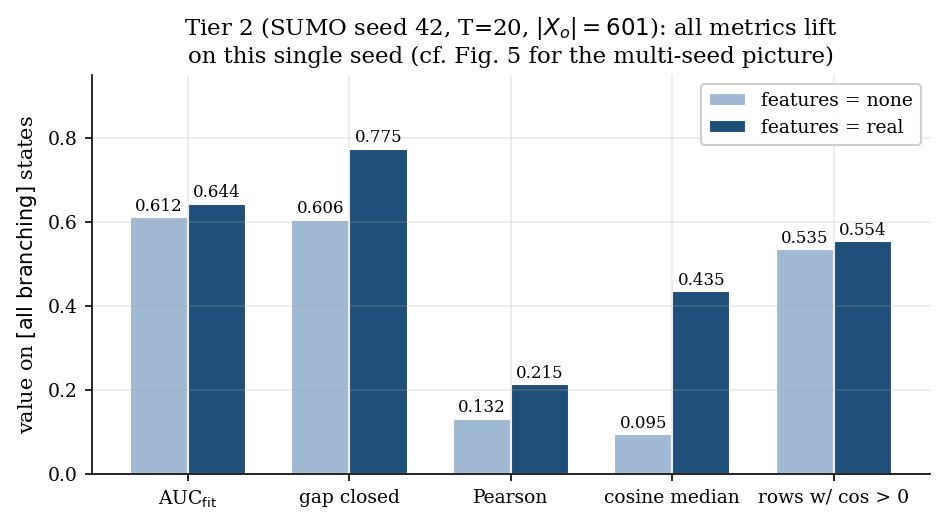
\includegraphics[width=0.95\linewidth]{fig03_phase4_features_lift.png}
\caption{Tier~2 features lift on the Ingolstadt SUMO network, seed~$42$, $T=20$.
Every metric, including detection AUC, gap-closed, per-row Pearson,
per-row cosine median and fraction of rows with positive cosine, moves
positively under \code{features=real} (dark) vs.\ \code{features=none}
(light). The Pearson +63\% relative lift and the cosine median
$4.6\times$ lift on the \texttt{[all branching]} generalisation block
are the strongest evidence that chain recovery, not aggregate-bias drift,
is what features improve.}
\label{fig:phase4-features-lift}
\end{figure}

\begin{table}[H]
\centering
\caption{Features lift across all metrics on the Ingolstadt SUMO network,
seed=42 (\cref{fig:phase4-features-lift}). \texttt{[all branching]}
restricts the per-row diagnostic to states with
$\mathrm{out\text{-}deg} > 1$ that the inverter did \emph{not} directly
observe, namely the generalisation block.}
\label{tab:phase4-features}
\small
\begin{tabular}{lccc}
\toprule
metric (\texttt{[all branching]}) & \texttt{features=none} & \texttt{features=real} & $\Delta$ \\
\midrule
$\AUC_{\mathrm{emp}}$ (full-obs.\ reference) & $0.685$ & $0.685$ & -- \\
$\AUC_{\mathrm{fit}}$ & $0.612$ & $\mathbf{0.644}$ & $+0.032$ \\
gap closed & $60.6\%$ & $\mathbf{77.5\%}$ & $+16.9$ pp \\
stacked Pearson($\Delta_{\mathrm{fit}}, \Delta_{\mathrm{emp}}$) & $+0.132$ & $\mathbf{+0.215}$ & $+63\%$ rel \\
per-row cosine median & $+0.095$ & $\mathbf{+0.435}$ & $4.6\times$ \\
rows with cosine $> 0$ & $53.5\%$ & $55.4\%$ & $+1.9$ pp \\
\bottomrule
\end{tabular}
\end{table}

Two results are worth separating. First, the $+0.032$ AUC lift on this
seed sits outside the single-instance variability measured in repeated
SUMO baseline runs. As the multi-seed
analysis of \cref{sec:phase4-multiseed} shows, however, this aggregate
AUC lift does \emph{not} survive replication across SUMO instances. The
per-row chain-recovery improvement, not the aggregate AUC, is the robust
effect. Second, the stacked Pearson on \texttt{[all branching]}
rises from $+0.132$ to $+0.215$, and the per-row cosine median from
$+0.095$ to $+0.435$. These are the metrics
that distinguish ``the fit improved because the chains got more accurate
per-row'' from ``the fit improved because the chains drifted in helpful
opposite directions in aggregate''. Both moved positively, supporting the
stronger chain-recovery claim. Unlike the aggregate AUC, this per-row
lift replicates across seeds (\cref{sec:phase4-multiseed}).

The one metric that barely moves is the fraction of rows with positive
cosine (only $+1.9$ pp on \texttt{[all branching]}, $58.6\%$ at
\texttt{[X\_o branching]}). Features sharpen the contrast magnitude in
the rows that were already approximately right, but do not flip the
sign on the $\sim 45\%$ of branching states whose fitted contrast points
the wrong way. This suggests the residual misspecification is
structural to the $1$-step softmax family. \Cref{sec:phase4-2step}
tests that hypothesis.

\subsubsection{Multi-seed validation: chain recovery is robust, detection AUC is not}
\label{sec:phase4-multiseed}

To test whether the seed-$42$ lift replicates, the contrast-correlation
diagnostic was run across five independent SUMO instances
(\code{randomTrips} seeds $\in \{7, 23, 42, 101, 2024\}$, observation-set
seed fixed at $13$, $T=20$, $|X_o|=601$, $\code{maxiter}=1500$) under both
\code{features=none} and \code{features=real}
(\cref{tab:phase4-multiseed}, \cref{fig:phase4-multiseed}).
Because the inverse-MC loss is non-convex, the optimiser can settle into
different local optima, or \emph{basins}, on different SUMO instances. A
basin here means a stable region of parameter space that L-BFGS-B reaches
and then cannot improve beyond, even though another instance may reach a
better region. The multistart audit in the Appendix tests whether random
re-initialisation can escape the low basin.

\begin{figure}[H]
\centering
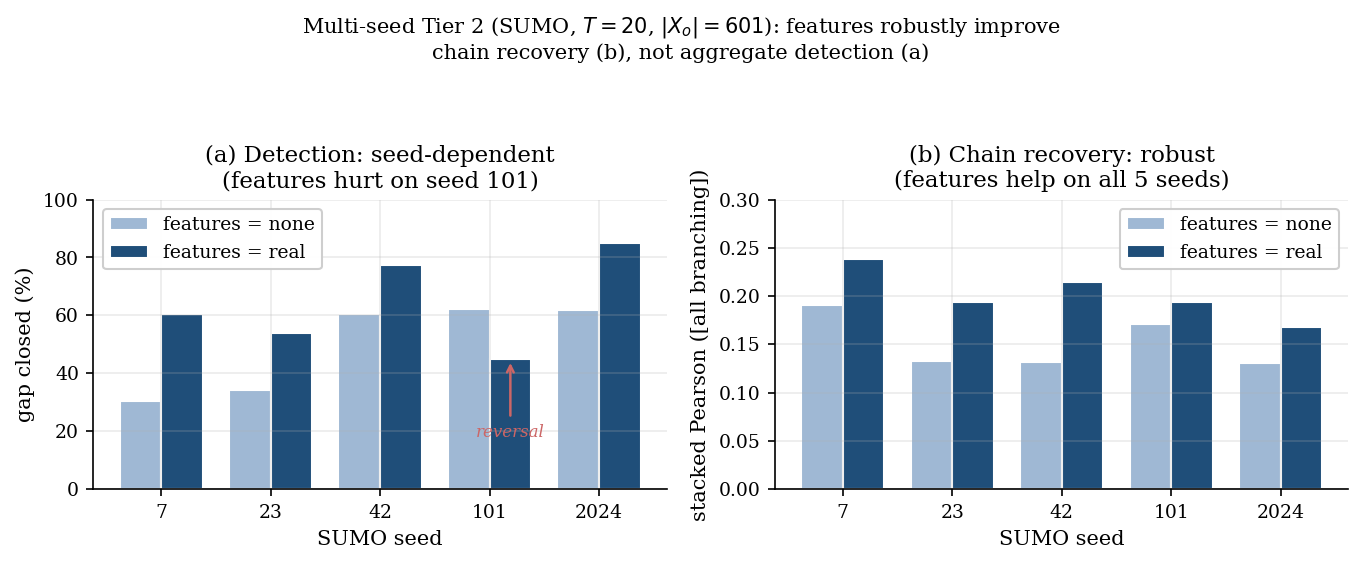
\includegraphics[width=0.98\linewidth]{fig05_phase4_multiseed.png}
\caption{Multi-seed Tier~2 features sweep (five SUMO seeds,
\texttt{[all branching]} block, $T=20$). \textbf{(a)} The aggregate
detection metric (gap-closed) lifts under \code{features=real} on four
seeds but \emph{reverses} on seed~$101$; the \code{features=none} bars
also reproduce the bimodal basin structure ($\{7,23\}$ low,
$\{42,101,2024\}$ high). \textbf{(b)} The per-row chain-recovery metric
(stacked Pearson) lifts on \emph{all five} seeds. Features are a robust
chain-recovery lever, not a robust aggregate-detection lever.}
\label{fig:phase4-multiseed}
\end{figure}

\begin{table}[H]
\centering
\caption{Multi-seed features sweep on the Ingolstadt SUMO network
(\cref{fig:phase4-multiseed}), \texttt{[all branching]} block,
$T=20$, $|X_o|=601$. The AUC lift reverses on seed~$101$; the Pearson
lift is positive on all five seeds. Mean~$\Delta$ rows are
\code{real}~$-$~\code{none} with sample standard deviation.}
\label{tab:phase4-multiseed}
\small
\begin{tabular}{lcccccc}
\toprule
 & \multicolumn{2}{c}{gap closed} & \multicolumn{2}{c}{$\AUC_{\mathrm{fit}}$} & \multicolumn{2}{c}{Pearson} \\
\cmidrule(lr){2-3}\cmidrule(lr){4-5}\cmidrule(lr){6-7}
seed & none & real & none & real & none & real \\
\midrule
$7$    & $30.3\%$ & $60.3\%$          & $0.544$ & $0.588$          & $+0.191$ & $+0.238$ \\
$23$   & $34.2\%$ & $53.8\%$          & $0.554$ & $0.585$          & $+0.133$ & $+0.194$ \\
$42$   & $60.6\%$ & $77.5\%$          & $0.612$ & $0.644$          & $+0.132$ & $+0.215$ \\
$101$  & $62.1\%$ & $\mathbf{45.0\%}$ & $0.581$ & $\mathbf{0.559}$ & $+0.171$ & $+0.194$ \\
$2024$ & $61.8\%$ & $85.1\%$          & $0.585$ & $0.618$          & $+0.131$ & $+0.168$ \\
\midrule
mean $\Delta$ & \multicolumn{2}{c}{--} & \multicolumn{2}{c}{$+0.024 \pm 0.026$} & \multicolumn{2}{c}{$\mathbf{+0.050 \pm 0.023}$} \\
\bottomrule
\end{tabular}
\end{table}

Three findings. First, the aggregate detection lift is \emph{not}
statistically robust: the paired $\AUC_{\mathrm{fit}}$ lift averages
$+0.024 \pm 0.026$ across the five seeds, positive on four but reversing
on seed~$101$ (a paired $t$-test gives $t \approx 2.0$, $p \approx 0.11$,
not significant at $\alpha = 0.05$). The single-seed $+0.032$ headline of
\cref{sec:phase4-features-result} is therefore a favourable draw, not a
replicable property of the aggregate AUC.

Second, the per-row chain-recovery metrics \emph{are} robust. The stacked
Pearson lift averages $+0.050 \pm 0.023$ and is positive on \emph{all five} seeds
($t \approx 4.9$, $p \approx 0.008$); the per-row cosine median lifts on
all five as well (mean $\approx +0.25$). Seed~$101$ is the clearest warning
that AUC and chain quality can move in different directions: features
\emph{hurt} its detection AUC ($0.581 \to 0.559$) while \emph{improving}
its chain recovery (cosine median $0.062 \to 0.475$). The features lever
is therefore a
\textbf{chain-recovery} improvement, not an aggregate-detection
improvement.

Third, the \code{features=none} fit reproduces the bimodal gap-closure
structure observed in repeated SUMO runs: seeds $\{7, 23\}$ cluster
low ($30$--$34\%$) and seeds $\{42, 101, 2024\}$ cluster high
($61$--$62\%$), with nothing in between. The same seeds fall in the same
clusters as the earlier run, indicating that the low/high split is a
property of the loss landscapes on these instances rather than measurement
noise. The \code{features=none} $\AUC_{\mathrm{fit}}$ across seeds is
$0.575 \pm 0.027$, consistent with the baseline variability. A follow-up
multistart audit tested whether the low basin could be escaped by random
re-initialisation; the detailed audit is reported in
Section~\ref{sec:phase4-multistart} in the Appendix, and it did not escape
the low basin.

\subsubsection{Higher-order memory diagnostic: a regularised 2-step
empirical lifts the reference}
\label{sec:phase4-2step}

A natural hypothesis for the still-flipped rows is that the $1$-step
Markov assumption is too forgetful. The fitted model sees only the current
edge $x_t$, but drivers may also condition on the edge they just came from:
``do not U-turn'', ``continue along the arterial'', or ``stay in this
lane group''. A $2$-step model gives the next-edge distribution the context
$(x_{t-1},x_t)$ instead of only $x_t$.

This subsection is a diagnostic, not a new fitted inverse-MC model. The
test is: if a full-observation empirical $2$-step scorer ranks the two
SUMO regimes better than the full-observation empirical $1$-step scorer,
then the data contain route-memory signal that the current $1$-step
softmax family cannot express. If it does not lift, the flipped rows are
more likely caused by optimisation, sparse observation, or feature
misspecification.

The catch is sparsity. On the Ingolstadt network the raw context space
$(x_{t-1},x_t)$ has roughly $|X|^2 \approx 5.8$M possible pairs, and most
possible pairs are never seen. A raw $2$-step empirical matrix would
therefore overfit rare contexts. Two regularisation schemes are tested
across the same five SUMO seeds used in \cref{sec:phase4-multiseed}
(training/test split unchanged):

\paragraph{Dirichlet smoothing: shrink rare contexts toward uniform turns.}
\[
\widehat{P}_{2,\alpha}(y | x_p, x) =
\frac{c(x_p, x, y) + \alpha}
{c(x_p, x) + \alpha \cdot |\mathrm{adj}(x)|},
\]
swept over $\alpha \in \{10^{-3}, 10^{-2}, 10^{-1}, 1, 10, 100\}$.

\paragraph{Interpolation backoff: shrink rare contexts toward the 1-step empirical.}
\[
\widehat{P}_{\mathrm{back}}(y | x_p, x) =
\lambda \cdot \widehat{P}_{2}^{\mathrm{MLE}}(y | x_p, x)
+ (1 - \lambda) \cdot \widehat{P}_{1}(y | x),
\]
where $\widehat{P}_{2}^{\mathrm{MLE}}$ is the unsmoothed 2-step MLE
and $\widehat{P}_{1}$ is the 1-step empirical chain that elsewhere
serves as the full-observation reference. Two $\lambda$ modes are tested:
\begin{itemize}
\item fixed $\lambda \in \{0, 0.25, 0.5, 0.75, 0.9, 1.0\}$;
\item count-conditional
$\lambda = N(x_p, x) / (N(x_p, x) + \kappa)$ with
$\kappa \in \{1, 10, 100, 1000\}$.
\end{itemize}
The count-conditional mode is the intuitive version: trust the $2$-step
estimate when a context has been seen often, and fall back smoothly to the
$1$-step empirical for rare contexts.

\begin{table}[H]
\centering
\caption{2-step empirical sweep on the Ingolstadt SUMO network across five SUMO seeds
($T=20$, training/test split as in \cref{sec:phase4-multiseed}, 1-step
empirical baseline mean $0.652 \pm 0.022$ across these seeds).
Each row reports the best configuration for that method. The single-seed
row is a comparison point; the multi-seed rows are the load-bearing
evidence.}
\label{tab:phase4-2step}
\scriptsize
\begin{tabular}{@{}p{0.27\linewidth}p{0.18\linewidth}ccc@{}}
\toprule
method & config & $\AUC_{\mathrm{2step}}$ & $\Delta$ & wins \\
\midrule
single-seed Dirichlet, seed~42 & $\alpha \to 0$ & $0.666$ & $-0.019$ & $0/1$ \\
\midrule
Dirichlet, multi-seed            & $\alpha = 10^{-3}$ & $0.673 \pm 0.012$ & $+0.021$ & $4/5$ \\
fixed backoff, multi-seed        & $\lambda = 0.9$    & $0.747 \pm 0.012$ & $+0.095$ & $5/5$ \\
\textbf{count backoff, multi-seed} & $\boldsymbol{\kappa = 100}$ & $\boldsymbol{0.752 \pm 0.015}$ & $\boldsymbol{+0.100}$ & $\boldsymbol{5/5}$ \\
\bottomrule
\end{tabular}
\end{table}

Three findings (\cref{tab:phase4-2step}).

First, the single-seed Dirichlet result is misleading. On seed~42 it gives
$0.666$, below the $1$-step reference of $0.685$, but seed~42 is also the
highest-reference seed in the sweep. There is less room to improve on
that seed than on the others. More importantly, Dirichlet smoothing
shrinks rare $2$-step contexts toward uniform outgoing turns, which throws
away useful $1$-step routing information.

Second, backoff to the $1$-step empirical is the right shrinkage target.
At $\kappa = 100$, the count-conditional rule gives positive lifts on all
five seeds, ranging from $+0.090$ to $+0.110$ (mean $+0.100$, standard
deviation $0.009$). On seed~42 the effective $\lambda$ across the
$3{,}528$ observed $(x_p,x)$ contexts has median $0.21$ and 10th--90th
percentiles $[0.03,0.81]$. In plain terms, the scorer mostly uses the
trusted $1$-step baseline and only lets the $2$-step context dominate
where the data support it.

Third, the conclusion is not sensitive to one hand-picked hyperparameter.
The fixed-$\lambda$ sweep gives lifts of
$+0.088$ to $+0.095$ for $\lambda \in \{0.25,0.5,0.75,0.9\}$, all
positive across all five seeds. The count-conditional sweep gives
$+0.095$ to $+0.100$ for $\kappa \in \{1,10,100,1000\}$. The exact
$+0.100$ maximum is mildly test-tuned, but the qualitative conclusion is
stable: any reasonable backoff strength lifts AUC by about $+0.09$ to
$+0.10$ across all five SUMO seeds.

\paragraph{Implication.} A properly regularised 2-step empirical
\emph{does} lift the reference, decisively, across every SUMO seed
tested: the regularised 2-step AUC reaches $0.752 \pm 0.015$ against
the 1-step baseline of $0.652 \pm 0.022$, a $+0.100$ delta whose
per-seed signs all point the same way. Two implications follow.

The per-row chain-recovery gap left by the $1$-step features lever
(\cref{sec:phase4-features-result}: $+0.215$ stacked Pearson on
\texttt{[all branching]}, $\sim 45\%$ of rows still with
wrong-direction contrast) is consistent with the $1$-step softmax
family being structurally unable to express $(x_{t-1}, x_t)$-conditional
choice. This is the regime where a parametric 2-step Morimura
extension is the right design lever, with the regularised empirical
sitting roughly $+0.10$ AUC above the 1-step reference at $T = 20$ as the
performance target it would need to approach.

No $\AUC_{\mathrm{fit}}$ is reported for the regularised
2-step diagnostic. A parametric 2-step Morimura inverter is a non-trivial
extension with a different state space, different gradient and different
reference argument, and is left to future work
(\cref{sec:disc-future}). The empirical result above establishes that
the signal exists and bounds the achievable 2-step inverter
performance from above; what it does not do is settle whether the
parametric inversion route can recover that bound under partial
observation.

\subsubsection{Trajectory-length sweep: lifting the reference and the detector together}
\label{sec:phase4-tsweep}

The $0.685$ reference is specific to the chosen test trajectory length
$T = 20$. The log-likelihood-ratio score $\Lam(\tau)$ is a sum of $T$
independent log-ratio increments, so its variance scales as $\sim T$.
Longer trajectories produce a tighter score distribution between the
two regimes and a higher achievable AUC; the data are ``the same'',
only the observation window is wider.

\begin{figure}[H]
\centering
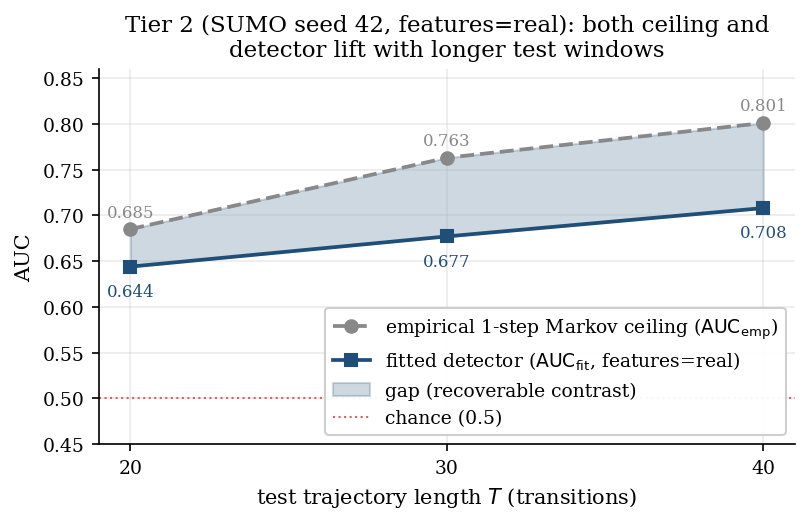
\includegraphics[width=0.78\linewidth]{fig02_phase4_tsweep.png}
\caption{Tier~2 $T$-sweep on the Ingolstadt SUMO network, seed~$42$,
\code{features=real}. The empirical $1$-step Markov reference
(grey dashed) rises with $T$ as expected for a variance-shrinking
score; the fitted detector (blue solid) tracks it with roughly constant
gap. The shaded region is the recoverable contrast not yet captured by
the fitter. The fitted chain itself is $T$-independent (identical final
losses across runs); only the trajectory-level scoring window changes.}
\label{fig:phase4-tsweep}
\end{figure}

\begin{table}[H]
\centering
\caption{$T$-sweep on the Ingolstadt SUMO network, seed=42, \code{features=real}
(\cref{fig:phase4-tsweep}). The fit itself is $T$-independent: only
the test scoring window changes, as confirmed by the identical
final-loss values $836.4 / 529.4$ across all three runs.}
\label{tab:phase4-tsweep}
\small
\begin{tabular}{ccccc}
\toprule
$T$ & $\AUC_{\mathrm{emp}}$ & $\AUC_{\mathrm{fit}}$ & gap closed & Pearson (all-br) \\
\midrule
$20$ & $0.685$ & $0.644$ & $77.5\%$ & $+0.215$ \\
$30$ & $0.763$ & $0.677$ & $67.4\%$ & $+0.220$ \\
$40$ & $\mathbf{0.801}$ & $\mathbf{0.708}$ & $69.0\%$ & $+0.216$ \\
\bottomrule
\end{tabular}
\end{table}

Two findings worth recording. First, the empirical reference rises from
$0.685$ to $0.801$ between $T=20$ and $T=40$, confirming that
the reference at $T=20$ was an artefact of the truncation window, not a
fundamental data limit. Second, the per-row Pearson is constant across
$T$ at $\sim +0.21$. $T$ is purely a scoring-window lever: it lets the
trajectory-level score discriminate more sharply, but it does not
change the chain that was fit. The fitted chain captures the same
$\sim 21\%$ of the true per-row contrast regardless of how long each test
trip is observed.

The strongest single-seed SUMO headline is therefore $\AUC = 0.708$
at $T=40$, $69\%$ of the gap closed against the full-observation
empirical $1$-step reference of $0.801$, with a stable per-row chain
Pearson of $+0.216$ on \texttt{[all branching]}.

A separate simulator stress test varied sat-navigation adoption and demand
independently before the rush-vs-off-peak proxy was used in Tier~3. The
full $\rho \times d$ decomposition is reported in
Section~\ref{sec:phase4-rho-demand} in the Appendix. In brief, under
SUMO's static unaided-driver baseline, changing demand alone produced a
near-random empirical AUC ($0.493 \pm 0.018$), while adding full
sat-navigation at peak demand produced a large signal
($0.780 \pm 0.013$). This supports the rush/off-peak proxy only as a weak
simulator audit: real commuters can remember recurring congestion, so the
real-world proxy may still mix human experience with algorithmic guidance.

\subsubsection{The \texorpdfstring{$f+g$}{f+g} extension at scale: a refined diagnosis}
\label{sec:phase4-fg-infeasible}

The optional $f+g$ loss was audited because the initial SUMO-scale run at
$|X_o|=601$ did not terminate after $9.5$ hours, but the diagnosis is more
specific than simple infeasibility. A finite-difference-verified sparse-LU
implementation confirms the mathematics, yet naive sparse solves are still
slower than dense at full SUMO scale because the wide gradient solve
dominates. On smaller Xuancheng subgraphs the solver is fast enough, but
a different problem appears: most observed station pairs are never hit, so
their empirical $g$ values sit at the same small floor. Intermediate
$\gamma$ then lets this low-information $g$ term overwhelm the useful
count signal $f$; only high-$\gamma$ settings close to the $f$-only end
recover the empirical reference. The practical detector in this
dissertation therefore remains $f$-only, and the solver profiling plus
$\gamma$ sweep are moved to Section~\ref{app:fg-profiling} in the
Appendix.

\subsection{Interpretation}

Tier~2 is the positive validation tier, but only under the controlled
conditions that make its labels meaningful. With ground-truth rerouting
labels and matched OD pairs, the fitted filter discriminates sat-navigation
from static unguided routing, reaching $\AUC=0.708$ at $T=40$ while
closing $69\%$ of the gap to the full-observation empirical $1$-step
reference. The feature-augmented score is useful primarily as a
chain-recovery lever: it improves per-row Pearson/cosine consistently
across five seeds, but its aggregate AUC lift is not robust.

The tier also identifies the model-class boundary. A regularised
empirical $2$-step reference lifts AUC by about $+0.09$--$+0.10$ on every
SUMO seed, showing that higher-order route memory is a real signal in the
controlled data and that a parametric $2$-step inverse-MC model is the
next justified detector design. By contrast, the $f+g$ extension is not
ready at city scale under the current solver: subgraph tests show that it
can help when $\gamma$ is tuned near the f-only end, but full-network
runtime and hitting-rate sparsity keep the deployed Tier~2 detector
f-only. The defensible claim from this tier is therefore specific:
the current $1$-step partial-observation filter works as a controlled
labelled detector, and its diagnostics correctly expose where richer
model structure is needed.


\section{Tier 3: Real-World Validation on Xuancheng AVI Data}
\label{sec:phase5-xuancheng}

This tier ports the entire pipeline to a real-world urban AVI dataset
from Xuancheng, China \cite{ma2026xuancheng}. The pipeline is unchanged
from Tier~2; only the loader and the regime split differ. The
methodological gap that distinguishes any real-world validation from
the controlled Tier~2 comparison --- namely, the absence of a
ground-truth sat-navigation adoption label --- is what we have to
address explicitly here.

\subsection{Dataset choice}\label{sec:phase5-dataset}

Three candidate datasets were evaluated. The Padua AVI deposit
\cite{cappi2026} releases only aggregated $10$-minute flow statistics
and pairwise travel times over $40$ junctions; per-vehicle trajectories
are stripped at the source pipeline for privacy and cannot be
reconstructed downstream. The Wang \emph{et al.}\ Xuancheng deposit
\cite{wang2023xuancheng} explicitly restricts raw trajectory access
behind a supervised-interactive interface. The
\citet{ma2026xuancheng} Xuancheng release, by contrast, publishes
joinable entry/exit tables with anonymised vehicle identifiers from
which complete per-vehicle trajectories can be reconstructed downstream;
this is the dataset we use. \cref{tab:phase5-dataset-scale} summarises
its scale.

\begin{table}[H]
\centering
\caption{Xuancheng AVI dataset \cite{ma2026xuancheng} scale, with comparison
to the SUMO bigger-bbox setup of Tier~2.}
\label{tab:phase5-dataset-scale}
\small
\begin{tabular}{lcc}
\toprule
property & SUMO bigger-bbox (Tier 2) & Xuancheng (Tier 3) \\
\midrule
state space $n$ & $2{,}405$ edges & $1{,}733$ edges (SCC subset) \\
trips per day & $\sim 28{,}000$ per regime & $\sim 327{,}000$ \\
mean trajectory length & $35.7$ edges & $15.1$ edges (raw) \\
total trips (full pool) & $\sim 56{,}000$ & $\sim 10.5$M (Apr 2023) \\
ground-truth regime label & yes (\code{rerouting} flag) & \emph{no} (proxy required) \\
\bottomrule
\end{tabular}
\end{table}

\subsection{Verification: route legality and time-of-day distribution}
\label{sec:phase5-verification}

Two non-obvious data-quality issues affect how the loader processes
trips, each of which was identified before any fitting was attempted:

\paragraph{Route legality.} Of all consecutive edge pairs $(x_t,
x_{t+1})$ across the trip routes, only $78.4\%$ satisfy the SUMO net's
lane-connection definition $x_{t+1} \in \mathrm{adj}(x_t)$. The
remaining $21.6\%$ split as $\sim 1.9\%$ junction-adjacent-but-disconnected
(a definitional gap in the converted SUMO net) and $\sim 19.7\%$
inter-junction ``teleports'' attributable to the source pipeline's
Dijkstra-repair step that fills in missing AVI passages on
CityFlow's connectivity graph rather than the SUMO net's. The loader
handles this by \emph{splitting trips at illegal boundaries} into
legal-only sub-trajectories rather than dropping the trip wholesale:
a $15$-edge raw trip with one illegal jump becomes two sub-trajectories.
Mean sub-trajectory length is $8.2$ edges, which caps the practical
test-window $T$ at $\le 10$.

\paragraph{Time-of-day distribution.} Across all $30$ daily files, the
trip \code{startTime} field is seconds-since-midnight in $[0, 86400]$
with a clear AM-rush + PM-rush + midday-off-peak structure. We use this
to construct a rush-vs-off-peak regime split with windows
$\text{rush} = [25{,}200, 32{,}400] \cup [61{,}200, 68{,}400]$
(7--9~AM and 5--7~PM) and
$\text{offpeak} = [36{,}000, 57{,}600]$ (10~AM--4~PM); trips outside
either window are discarded. Three anomalous days are flagged for
exclusion or special handling: Apr~5 (Tomb-Sweeping holiday, $264$k
trips, demand outlier), Apr~28--29 (Labour Day eve, $\sim 425$k trips),
Apr~10 (\code{startTime} max~$\approx 165$k, suggesting a multi-day
concatenation), and Apr~8/9 (identical trip counts of $324{,}441$ in both
files, almost certainly a duplicate).

\subsection{The fundamental real-world gap: no ground-truth sat-nav label}
\label{sec:phase5-proxy}

Tier~2 used \code{--device.rerouting.probability} as ground truth: every
vehicle either does or does not use sat-navigation, and the regime split
is exact by construction. No real-world AVI dataset publishes this
label. The closest behavioural proxy available in Xuancheng is the
rush-vs-off-peak time-of-day contrast: if external rerouting influence
is triggered by congestion, then rush-hour trips should differ from
off-peak trips in routing choices, and the inverse-MC detector should
detect that difference.

This proxy is weaker than the SUMO contrast in two ways. First, rush
and off-peak trips have \emph{different populations} (commuters vs.\
discretionary trips), so any chain difference reflects both the
routing-choice effect (which we want) and the OD-mix effect (which
we do not). Second, the actual sat-navigation adoption rate in
Xuancheng is presumably much lower than the $100\%$ used in SUMO, so
even the routing-choice signal is diluted by the unguided fraction.

We address the OD-mix confound directly via the OD-rebalancing
extension of \cref{sec:od-rebal}. We cannot address the lower-adoption
dilution from observation alone; what we can do is report the resulting
real-world AUC honestly as a lower bound on the method's sensitivity
in deployment.

\subsection{Results}\label{sec:phase5-results}

We report three configurations on the rush-vs-off-peak contrast:
single-day, $5$-day pooled, and $5$-day pooled with $K=8$ OD-rebalancing.

\begin{figure}[H]
\centering
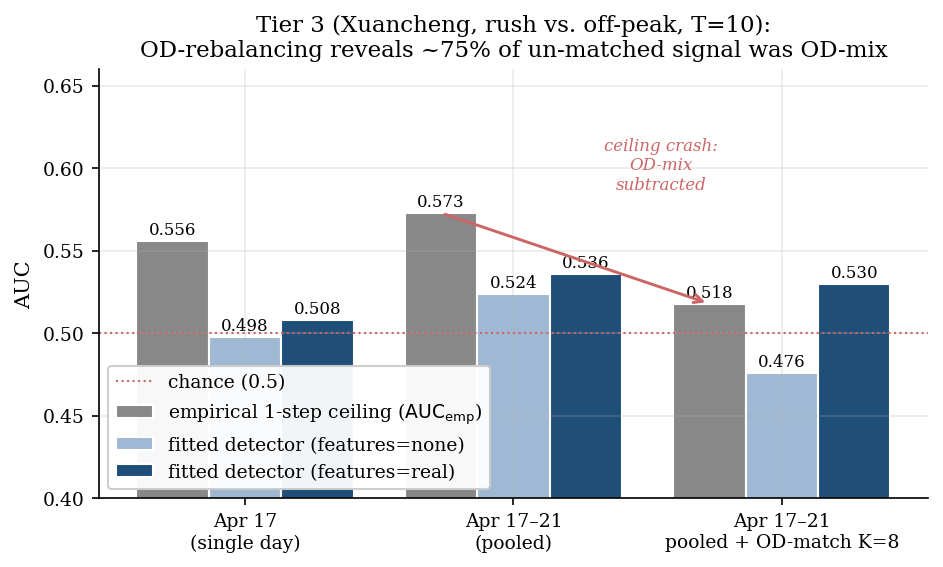
\includegraphics[width=0.95\linewidth]{fig04_phase5_xuancheng.png}
\caption{Tier~3 Xuancheng rush-vs-off-peak detection AUC across three
configurations. The empirical $1$-step Markov ceiling (grey) is
$0.556$ on a single day, lifts to $0.573$ when $5$ weekdays are pooled,
and \emph{crashes} to $0.518$ once the pools are OD-matched at $K=8$
spatial zones. The $0.055$ AUC drop attributable to the OD-rebalancing
identifies approximately $75\,\%$ of the un-matched detection signal
as origin-destination-mix between commuter and discretionary trip
populations, not routing-choice differences. Fitted detectors
(blue bars) follow the ceiling in all three configurations.}
\label{fig:phase5-headline}
\end{figure}

\begin{table}[H]
\centering
\caption{Xuancheng rush-vs-off-peak detector AUC and chain-recovery
metrics on \texttt{[all branching]} states, three configurations
(\cref{fig:phase5-headline}).}
\label{tab:phase5-headline}
\small
\begin{tabular}{lcccc}
\toprule
configuration & $\AUC_{\mathrm{emp}}$ & $\AUC_{\mathrm{fit}}$ \footnotesize{(none/real)} & Pearson \footnotesize{(none/real)} & median cos \footnotesize{(none/real)} \\
\midrule
day=Apr~17, T=10 & $0.556$ & $0.498 / 0.508$ & $+0.139 / +0.048$ & $+0.341 / +0.146$ \\
pool Apr~17--21, T=10 & $0.573$ & $0.524 / 0.536$ & $+0.096 / +0.072$ & $+0.267 / +0.167$ \\
pool + OD-match $K=8$ & $\mathbf{0.518}$ & $0.476 / 0.530$ & $+0.104 / +0.077$ & $+0.332 / +0.263$ \\
\bottomrule
\end{tabular}
\end{table}

The critical row is the third. The OD-rebalancing step matches $517{,}477$
trips per regime across $55$ shared $(\text{zone}_o, \text{zone}_d)$
cells (only $1$ OD cell out of $56$ was rush-only or off-peak-only,
discarded), removing the OD-mix confound. The empirical ceiling
\emph{crashes} from $0.573$ to $0.518$ --- i.e.\ only $0.018$ above
chance. This is the methodologically central number of the real-world
tier: approximately $75\%$ of the rush-vs-off-peak detection
signal visible in the un-matched pool is attributable to the OD-mix
\emph{not} to routing differences. After controlling for it, the
within-OD routing contrast is essentially absent at the $1$-step
Markov level in this dataset.

A secondary observation: in the OD-matched row, $\AUC_{\mathrm{fit}}$
under \code{features=real} ($0.530$) numerically exceeds
$\AUC_{\mathrm{emp}}$ ($0.518$). Under correct chain recovery this is
impossible, since the full-observation empirical chains should upper-bound
any partial-observation fit. The most plausible explanation is the
same L-BFGS basin-selection pathology that hit the un-matched pool
(rush-fit loss spikes from $4.058$ at \code{features=none} to $1397$ at
\code{features=real}, a $\sim 340\times$ ratio); the resulting fitted
chains drift in directions that happen to produce a slightly better
aggregate-bias signal than the empirical chains, but not because they
are more chain-accurate. The per-row Pearson on \texttt{[all branching]}
of $+0.077$ (real) vs $+0.104$ (none) under OD-matching corroborates
this: features make chain recovery slightly \emph{worse}, not better,
on real data with this loss landscape.

\subsection{Honest reading}\label{sec:phase5-reading}

Three findings are worth foregrounding from \cref{tab:phase5-headline}.

\paragraph{The OD-mix dominates the un-matched signal.} The empirical
ceiling falls from $0.573$ (un-matched pool) to $0.518$ (matched
pool); $0.055$ AUC of the un-matched signal --- approximately $75\%$
of the above-chance ceiling at $0.073$ --- is the OD-mix confound. The
remaining $0.018$ AUC above chance is the genuine routing-given-OD
contrast at the $1$-step Markov level. This is the central
methodological point of the real-world tier: \emph{without} OD-matching,
a method appears to detect ``rush-hour routing differences''; \emph{with}
OD-matching, it correctly attributes most of that apparent signal to
the trivially expected fact that commuters and discretionary travellers
have different origin-destination distributions.

\paragraph{The within-OD routing contrast is below detectability.}
At the OD-matched ceiling of $0.518$ ($0.018$ above chance), the
fitted detectors at $0.476$/$0.530$ are not meaningfully distinguishable
from chance under any plausible single-seed noise band. Per-row
Pearson on \texttt{[all branching]} is $\le 0.104$ in every Xuancheng
configuration, against $+0.215$ on SUMO under labelled comparison.
Whatever real congestion-induced rerouting exists in Xuancheng at
April 2023 sat-navigation adoption rates is below the $1$-step Markov
behavioural-proxy detection threshold of this framework.

\paragraph{The features=real basin failure repeats post-matching.} Both
the un-matched pool (\cref{sec:phase5-results}) and the OD-matched pool
show the same pattern: the rush-fit \code{features=real} loss is
$\sim 350\times$ the \code{features=none} loss
($1397$ vs.\ $4.058$ here). The $\AUC_{\mathrm{fit}} > \AUC_{\mathrm{emp}}$
behaviour in the matched row is consistent with this being a
basin-selection artefact rather than a chain-recovery improvement. A
multistart $K \ge 5$ run is the obvious diagnostic; it is flagged as
immediate future work and not run here.

\subsection{Bottom line for Tier 3}\label{sec:phase5-bottom}

The pipeline runs cleanly on real-world data. The framework's
gradient implementation, FD-check, regime-split machinery, and contrast
diagnostics all port to the Xuancheng dataset without modification, and
the OD-rebalancing extension cleanly attributes the un-matched pool's
apparent signal to its sources. The headline finding is that
\textbf{approximately three-quarters of the un-matched rush-vs-off-peak
detection signal in Xuancheng is OD-mix, not routing}; the remaining
routing-given-OD contrast is only $0.018$ AUC above chance and is below
the detectability threshold of a $1$-step Markov framework applied to
this behavioural proxy. This is a methodologically strong negative
result for behavioural-proxy validation of sat-navigation detection
on real-world AVI data, and it explicitly characterises the gap between
the controlled-simulation regime (Tier~2, $0.708$ AUC on labelled
SUMO contrast) and the real-world regime under realistic
sat-navigation adoption rates.

The result also identifies the methodological lever any future
real-world validation of this framework needs: \emph{ground-truth
sat-navigation adoption labels}, even partial, on the underlying trip
records. With them, the proxy-weakness problem disappears and the
controlled-comparison machinery of Tier~2 transfers directly. Without
them, behavioural proxies appear systematically to over-estimate the
real-world detection signal once OD-mix is controlled for.


\section{Discussion}\label{sec:discussion}

\subsection{Cross-tier comparison}
\label{sec:disc-cross-tier}

The core inverse-MC scoring machinery works cleanly across all three
tiers: the inverter, FD-checked gradient, contrast diagnostic, and
feature plumbing operate unchanged on a synthetic $n=100$ chain, a SUMO
$n=2{,}405$ network, and a real-world $n=1{,}733$ Xuancheng network. What
differs by tier is the loader, the regime definition, and the
OD-control logic; the shared scoring core is selected by a single
\code{--dataset \{sumo,xuancheng\}} command-line interface (CLI) flag. This is a useful
generalisation result for an inverse-MC pipeline that the original paper
validated only on synthetic data and one real-world demonstration.

What does not generalise as cleanly is the magnitude of the
detection signal. Tier~1 reproduces the paper's RMAE within
$\sim 0.05$ for $|\Xo| \ge 10$. Tier~2 reaches $\AUC = 0.708$ at $T=40$
on the controlled SUMO comparison, $\sim 69\%$ of the gap to the
full-observation empirical $1$-step reference of $0.801$, with per-row
chain Pearson $\sim +0.21$. Tier~3 on Xuancheng, with no ground-truth
sat-navigation label, gives chance-level fitted AUC on the
rush-vs-off-peak behavioural proxy. A stronger Labour-Day proxy creates
a significant fine-OD empirical signal ($\AUC_{\mathrm{emp}}=0.567$),
but multistart validation-selected fitting still falls to chance
($\AUC_{\mathrm{fit}}=0.502$). The drop
between Tier~2 and Tier~3 has two distinct contributions:
\begin{itemize}
\item The Xuancheng ceiling itself ($\AUC_{\mathrm{emp}} \sim 0.57$) is
much lower than the SUMO ceiling ($\sim 0.69$), reflecting that the
behavioural rush-vs-off-peak proxy is a weaker contrast than the
SUMO labelled comparison.
\item Xuancheng is also scored on shorter legalised trajectories
($T=10$), whereas the main SUMO detector starts at $T=20$ and improves
again at $T=30$ and $T=40$. Since the LLR score accumulates evidence over
the trajectory, the shorter real-data window likely suppresses both the
empirical reference and fitted AUC.
\item The fitted-vs-reference gap is not merely a scaled-down
version of the SUMO success. The pooled un-matched Xuancheng row gives
a superficially moderate gap-closure number because the reference itself
is weak, but once OD mix is controlled the fitted detector sits at chance
across every tested $K$ while the full-observation reference remains
weakly above chance at finer granularities. Tier~3 is therefore a
negative result for the current $1$-step partial-observation filter
under this behavioural proxy.
\item The Labour-Day stress test rules out the strongest alternative
reading: that a more intuitive real-world contrast would rescue the
detector. Labour Day does yield a stronger empirical reference after
fine OD matching, but the fitted chain remains near chance and multistart
selection removes the small zero-init lift.
\item A fitting-free $2$-step backoff audit on the same Labour-Day split
also fails to lift the empirical reference: the best setting is the
degenerate $\lambda=0$ backoff, equivalent to the original $1$-step
chain. The SUMO route-memory result therefore motivates a future model
class, but it is not by itself an explanation of the Xuancheng failure.
\end{itemize}
Under controlled labelled simulation the method recovers a robust
fraction of the per-row chain contrast. On a real-world behavioural
proxy, the fitted $1$-step detector remains near chance once
population-mix is controlled.

\Cref{tab:cross-tier} consolidates the three tiers on a common axis:
the same inverter and diagnostic produce every row, and the trend in the
empirical ceiling, from a noise-free synthetic recovery, through a
labelled simulated comparison, to a behavioural real-world proxy,
quantifies how much detectable signal each setting actually contains.

\begin{table}[H]
\centering
\caption{Cross-tier synthesis. Tier~2 reports the representative
Ingolstadt seed~$42$ at $T=20$; Xuancheng rows report the weekday proxy
and the Labour-Day stress test. Fitted and Pearson cells are
\code{none}/\code{real}.}
\label{tab:cross-tier}
\scriptsize
\setlength{\tabcolsep}{3pt}
\begin{tabular}{@{}p{0.17\linewidth}p{0.23\linewidth}ccc@{}}
\toprule
tier & dataset ($n$) & empirical ceiling & fit AUC & Pearson \\
\midrule
1 synthetic              & random graph ($100$)  & --     & --             & -- \\
2 SUMO                   & Ingolstadt network ($2{,}405$) & $0.685$ & $0.612 / 0.644$ & $+0.132 / +0.215$ \\
3 Xuancheng              & AVI ($1{,}733$)        & $0.573$ & $0.524 / 0.536$ & $+0.096 / +0.072$ \\
3 Xuancheng Labour       & AVI ($1{,}733$)        & $0.567$ & $0.521 \rightarrow 0.502$ & $+0.066$ \\
\bottomrule
\end{tabular}
\end{table}

\subsection{Limits of the chosen approach}
\label{sec:disc-limits}

The main limitations are label availability, stationarity, and model
capacity.

\paragraph{Proxy labels and stationarity.} Tier~3 cannot observe
sat-navigation use directly, so rush-vs-off-peak and Labour-Day splits
are behavioural proxies. They mix route guidance, ordinary congestion
adaptation, driver composition and OD mix. The estimator also compresses
dynamic time windows into one stationary surrogate chain, which is useful
for scoring but should not be interpreted as a literal invariant traffic
distribution.

\paragraph{Controlled simulation versus real traffic.} Tier~2 provides a
labelled test bed, yet it still contains simulator-specific structure:
at the selected demand the sat-navigation regime completes many more
trips, and unaided SUMO drivers follow precomputed routes. The
$\rho \times d$ audit in Section~\ref{sec:phase4-rho-demand} in the
Appendix shows that this simulator signal is mainly tied to the
sat-navigation label, but a real experienced driver can adapt without
live route guidance. This is why Tier~3 remains a proxy stress test until
trip-level guidance labels are available.

\paragraph{Sparse observation, optimisation and feature capacity.} Both
SUMO and Xuancheng show that the inverse problem is under-constrained at
city scale. Multi-seed SUMO runs make the feature result weaker as an AUC
claim but robust as a per-row chain-recovery effect; Xuancheng multistart
removes an apparent \code{features=real} ceiling violation and returns the
fitted detector to chance. The $f+g$ extension adds another capacity
route, but its city-scale implementation remains expensive because each
iteration needs large linear solves. The current thesis therefore uses
the tractable $f$-only detector and treats $f+g$ and higher-order dynamics
as model-class extensions.

\subsection{Social, environmental, technological implications}
\label{sec:disc-implications}

\paragraph{Transport-policy modelling.} Navigation platforms can change
the routes that appear in revealed-preference data. If those influenced
routes are fed back into demand models as ordinary preferences, policy
evaluation can confuse platform response with driver preference. The
controlled SUMO result shows that inverse-MC filtering can recover part
of this distinction when labels exist; the Xuancheng result shows that
behavioural proxies alone are too weak for confident attribution.

\paragraph{Privacy and data access.} The evidence needed for this task is
awkward: trip-level trajectories are useful, but trip-level app-use labels
are sensitive. Aggregate-only releases protect privacy but cannot support
the detector tested here; joinable per-trip releases enable the method
while increasing reidentification risk. A practical deployment would need
privacy-preserving access to coarse guidance/compliance labels, or a
trusted-analysis setting in which labels can be used without publishing
raw identifiers.

\paragraph{Platform accountability.} A reliable detector would let cities
audit how much of observed route choice is shaped by guidance systems,
without needing to inspect individual recommendations. This matters for
congestion pricing, traffic-calming decisions and claims about network
welfare. The negative Tier~3 result is part of that accountability story:
it warns against treating rush-hour AVI contrasts as evidence of
sat-navigation influence unless the proxy is supported by labels or a
stronger behavioural model.

\subsection{Future work}
\label{sec:disc-future}

\begin{enumerate}
\item \textbf{Labelled real-world validation.} The highest-value next
dataset would pair trajectories with coarse sat-navigation-use or
route-guidance-compliance labels. Even partial labels would convert
Tier~3 from a proxy stress test into a direct validation exercise.

\item \textbf{Robustness over stations, OD cells and cities.} The current
fits condition on one observation-station set and a fixed OD match. A
deployment study should repeat the inverse-MC fits over multiple $\Xo$
draws, resample OD cells, and replicate across more city/month pools.

\item \textbf{Richer behavioural state.} SUMO shows that second-order
route memory can carry signal, while Xuancheng Labour does not show a
simple empirical $2$-step lift. A parametric extension should therefore
test higher-order context, time-of-day conditioning and trip-level
features as competing explanations, with the chain-recovery claim kept
separate from any deployment-oriented classifier.

\item \textbf{Scalable $f+g$ optimisation.} The hitting-rate extension
remains attractive because it uses more of Morimura's original evidence,
but city-scale fitting needs factor sharing or a different optimiser.
Sherman--Morrison updates for the $(I-\beta P_T)$ solves and
natural-gradient or Levenberg--Marquardt steps are the most direct
algorithmic candidates.

\item \textbf{Experienced-driver simulation.} The Tier~2
$\rho \times d$ decomposition should be repeated with unaided drivers who
avoid known rush-hour bottlenecks. That counterfactual would make the
simulator bound closer to the real Xuancheng ambiguity between human
experience and algorithmic guidance.
\end{enumerate}


\section{Conclusion}\label{sec:conclusion}

This dissertation designed and audited a
\emph{partial-observation routing-influence filter}. The filter ingests a
road graph, sparse regime-labelled station observations at $\Xo$, and
held-out trajectories; it fits one inverse-Markov-chain model per regime;
then it scores each trajectory with a log-likelihood ratio. The underlying
estimator is Morimura et al.'s inverse-MC method~\cite{morimura2013}; the
contribution here is the two-regime detector built around it, the
trajectory-level scoring rule, and the diagnostic suite used to decide
whether a positive AUC is actually evidence of route-choice recovery.

\paragraph{What the evidence supports.}
Tier~1 validates the estimator implementation: on Morimura et al.'s
synthetic recovery benchmark, the reproduced RMAE curve tracks the
published proposed-method curve for $|\Xo|\ge10$, with analytic gradients
finite-difference checked before downstream use. Tier~2 is the positive
detector result. In labelled SUMO simulation, with shared OD pairs and a
known rerouting flag, the filter reaches $\AUC=0.708$ at $T=40$ against a
full-observation empirical $1$-step reference of $0.801$. The
feature-regularised variant does not robustly lift aggregate AUC across
all seeds, but it does robustly improve per-row chain recovery, which is
the stronger claim. Tier~3 is the real-world stress test. On Xuancheng AVI
data, where only behavioural proxy labels are available, the fitted
$1$-step detector remains near chance after OD control: rush-vs-off-peak
does not recover at any tested OD granularity, and the stronger
Labour-Day-vs-normal split falls to $\AUC=0.502$ under
validation-selected multistart despite a weak full-observation empirical
signal.

\paragraph{What the audits changed.}
Several headline-looking results became more precise once audited. The
SUMO features result became a chain-recovery result rather than a robust
detection-AUC result. The SUMO $2$-step empirical backoff lifted AUC by
about $+0.09$--$+0.10$ across all five seeds, showing that higher-order
route memory is a real signal in the controlled data and a justified
future model class. The same $2$-step audit did not help on the Xuancheng
Labour-Day split, so route memory is not the simple missing lever for that
real-world proxy. The optional $f+g$ route is mathematically verified and
useful on small subgraphs when $\gamma$ is tuned near the $f$-only end, but
naive city-scale sparse-LU is too slow and empirical hitting rates are too
floor-dominated to use as the deployed full-network detector in this
thesis.

\paragraph{Where the filter is reliable.}
The filter is reliable as a controlled labelled detector under the
conditions tested in SUMO: matched OD pairs, known rerouting labels, and a
finite-data empirical reference against which chain recovery can be
audited. In that setting it recovers a substantial fraction of the
available $1$-step signal and exposes where the $1$-step model class runs
out of capacity.

\paragraph{Where it is not reliable.}
The filter does not support a positive real-world sat-navigation detection
claim on Xuancheng. Without trip-level guidance/adoption labels,
rush-vs-off-peak and Labour-Day splits remain behavioural proxies that mix
route guidance, ordinary congestion adaptation, driver composition, OD
mix, time heterogeneity and data-quality effects. Once those confounds are
audited, the fitted partial-observation detector does not robustly recover
the within-OD signal that remains in the full-observation reference.

\begin{figure}[H]
\centering
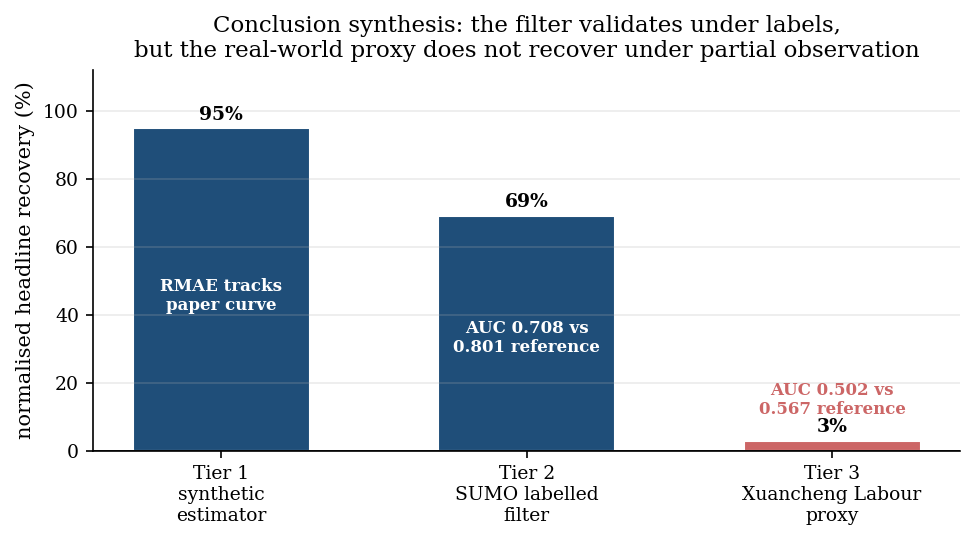
\includegraphics[width=0.92\linewidth]{fig08_conclusion_synthesis.png}
\caption{Cross-tier synthesis of the dissertation's headline results.
The bars use a normalised summary, since the tiers use different metrics:
Tier~1 reports benchmark-reproduction closeness, computed as the mean
capped ratio between the visual paper RMAE and this reproduction's RMAE for
$|\Xo|\ge10$; Tiers~2--3 report AUC gap closed,
$(\AUC_{\mathrm{fit}}-0.5)/(\AUC_{\mathrm{emp}}-0.5)$. The central pattern
is that the estimator reproduces its synthetic benchmark, the labelled
SUMO filter recovers a substantial fraction of the empirical $1$-step
signal, and the real Xuancheng behavioural proxy does not recover under
the fitted partial-observation model.}
\label{fig:conclusion-synthesis}
\end{figure}

The practical conclusion is therefore sharper than a single AUC number:
the inverse-MC machinery is not the main bottleneck for real-world
externally-influenced routing detection. The bottleneck is validation
data. A future deployment needs at least partial trip-level
sat-navigation-use or guidance-compliance labels, repeated station and OD
sensitivity checks, and a richer model class where the controlled data
show it is warranted. Until those labels exist, this framework is best
read as a validated controlled-simulation filter and a real-world
confounding audit, not as a finished real-world sat-navigation detector.


\section{Project Management and Reflection}\label{sec:reflection}

\subsection{Project structure and milestone management}
\label{sec:reflect-pm}

The project was scoped at the outset as a three-tier validation
pipeline (synthetic, simulated, real-world) extending a single source
paper \cite{morimura2013}. This decomposition gave the work a useful
order: first verify the estimator on the paper's own benchmark, then test
the full detector in labelled simulation, then stress-test the same
pipeline on real data where the labels are only proxies.

Milestone management was driven by a continuously updated
\code{research\_logbook.md}. After each experimental cycle I recorded the
hypothesis, setup, result, interpretation, and next action. The logbook
became especially useful when results changed direction: it made it clear
which claims were still supported by evidence and which were only working
assumptions from an earlier stage.

Two practices worked well:
\begin{itemize}
\item \textbf{Audit-before-extend.} An early retraction of a headline
number made it clear that every extension needed an upstream audit first.
The gradient finite-difference check at $\sim 10^{-9}$ relative error
confirmed the analytic gradient derivation before the feature sweep, and
the contrast-correlation diagnostic showed that AUC alone was not enough
to claim chain recovery.
\item \textbf{Keeping decisions traceable.} Linking each reported number
back to a script, seed, log entry and interpretation note made the late
rewrite possible. It was particularly important for the $f+g$ diagnosis,
the SUMO multistart check and the Labour-Day stress test, all of which
changed how the results should be framed.
\end{itemize}

Two practices that did not work as well are worth recording explicitly:
\begin{itemize}
\item \textbf{Underestimating the compute scaling of the $f+g$ loss.}
The first $f+g$ sweep at SUMO scale was projected at $\sim 1$ hour and
killed at $9.5$ hours. The retry at smaller $|X_o|$ and
$\code{maxiter}$ was projected at $\sim 30$ minutes and killed at
$3$~hours. Two iterations were burned before the structural
diagnosis (the hitting-rate gradient is $O(|X_o| \cdot n^3)$ and the
$84\%$-floor loss landscape is degenerate at this scale) was reached.
In future I would profile a single iteration before committing to a
sweep at unfamiliar configuration.
\item \textbf{Late identification of the OD-mix confound.} The Tier-3
rush-vs-off-peak proxy was scoped before the methodological cost of
the OD-mix confound was clearly understood. The OD-rebalancing
extension, the methodologically correct fix, was added late in the
project, and the matched-pool result it produced
(\cref{sec:phase5-interpretation}) materially changed the Tier-3 interpretation.
Earlier scoping would have caught this; the lesson is that
``proxy weakness'' should be a structured pre-experiment audit item,
not an ad-hoc discussion item.
\end{itemize}


Looking back, the strongest parts of the project are the staged
validation structure and the willingness to keep negative results in the
main argument. The work did not stop at reproducing the source paper: it
tested the estimator inside a detector, separated labelled simulation from
proxy-labelled real data, and used diagnostics to avoid over-reading a
single AUC. The main weaknesses are also clear. Tier~3 uses one real
city/month pool rather than multiple independent real-world replications,
and the feature result that first looked like a detection improvement
became seed-dependent once the full SUMO sweep was run.

\subsection{Personal skill development}
\label{sec:reflect-skills}

The technical skills I leaned on heavily and improved in: deriving and
finite-difference-verifying analytic gradients (Eqs.~12, 15, 17--18 of
the source paper); writing software with a clean separation between
the inverter's mathematical core (in \code{morimura.py}, kept faithful
to the paper) and the application-specific loaders that surround it
(\code{sumo\_to\_phase3.py}, \code{real\_data/load\_xuancheng.py});
and writing a logbook that records both the successful and the
unsuccessful experimental cycles in enough detail that I could
critique my own past decisions a month later.

The non-technical skill I would name as the one that most shaped the
project's outcome is \emph{disciplined treatment of negative results}. The
project did not produce the headline ``real-world detector with a
high AUC and clean chain recovery'' that the SUMO Tier-2 result would
have predicted. Instead it produced: a controlled-validation result
($\sim 0.71$ AUC, $69\%$ gap closure on labelled SUMO), a model-class
diagnostic (the empirical $2$-step detector improves the $1$-step
reference, strengthening the case for a parametric $2$-step
extension), and a real-world result ($\sim 0.53$ AUC on a
behavioural proxy without ground-truth labels) that quantifies the gap
between simulated and real-world detectability. Each of these is a
methodologically useful result, in part because they were framed
accurately. The temptation late in the project to treat a stronger
holiday proxy as a headline rescue had to be handled carefully rather
than either embraced uncritically or dismissed. Running it with the same
OD controls, bootstrap intervals, per-row diagnostics and multistart
audit showed the useful version of the negative result: Labour Day has a
real full-observation within-OD signal, but the fitted detector still
falls to chance under validation-selected multistart. Accepting that
result, rather than chasing a higher headline number, is the skill I most
want to carry forward.


% ----------------- References -------------------------------------------------
\newpage
\bibliography{references}

% ----------------- Appendices -------------------------------------------------
\appendix
\section{Repository structure and reproducibility}
\label{app:repo}

The codebase is organised as follows.

\begin{description}
\item[\code{morimura.py}] The inverter core: \code{Inverter} class with
softmax-parametric chain, analytic gradients (local + globals),
$\lambda$-cross-validated fit, and the synthetic $\S 6.1$ reproduction
driver.
\item[\code{congestion\_filter.py}] Early exploratory experiments:
snapshot-level
two-regime synthesis and detection.
\item[\code{per\_car\_detector.py}] Tier-2 per-trajectory log-likelihood-ratio detector.
\item[\code{sumo\_validation/}] The SUMO-side machinery:
\code{sumo\_to\_phase3.py} (network builder, trip reader, feature
extractor), \code{score\_seed\_big.py} and \code{contrast\_correlation.py}
(scorers, with the \code{--dataset \{sumo,xuancheng\}} switch),
the empirical and backoff $2$-step diagnostics
(\cref{sec:phase4-2step,sec:phase5-labour}), and
\code{fd\_check\_features.py} (the FD gradient gate). Exact script names
and log paths are indexed in \code{sumo\_validation/README.md}.
\item[\code{real\_data/}] The Xuancheng tier: the unmodified
\code{xuancheng.net.xml} from \cite{ma2026xuancheng}, the daily JSON
trip files, and \code{load\_xuancheng.py} which provides the loader,
the three regime-split helpers, and the OD-rebalancing extension.
\item[\code{papers/}] Source PDFs of all cited works.
\item[\code{research\_logbook.md}] The day-by-day project log,
with twenty experimental-cycle entries.
\end{description}

\section{Use of generative AI}\label{app:ai}

In accordance with the module's declaration requirement, generative AI
was used in this project as follows. LLM-based code assistants,
including Claude, Codex and Gemini, were used as pair-programming and
writing-support aids throughout the implementation and writeup phases:
drafting code (with the author's careful review of every line before
commit), writing unit-test scaffolding, deriving analytic gradient
formulas alongside the author, checking mathematical and experimental
arguments, and helping edit the report for clarity. The author retained
responsibility for the research design, interpretation, code accepted
into the repository, and final submitted text.

\section{Build and reproducibility}\label{app:build}

The project is reproducible from the repository via the README, with
the following minimum environment:

\begin{lstlisting}[language=bash]
# Python 3.14, see project README
python3 -m venv .venv
.venv/bin/python -m pip install numpy scipy matplotlib

# Tier 1: synthetic Morimura reproduction (~20 s)
.venv/bin/python morimura.py

# Tier 2: SUMO experiments (requires SUMO_HOME set)
.venv/bin/python sumo_validation/contrast_correlation.py \
    --seed 42 --features real --T 40 --maxiter 1500

# Tier 3: Xuancheng experiments (requires real_data/ populated)
.venv/bin/python sumo_validation/contrast_correlation.py \
    --dataset xuancheng \
    --day 2023-04-17,2023-04-18,2023-04-19,2023-04-20,2023-04-21 \
    --regime_split rush_offpeak --od_match 8 \
    --features real --T 10 --maxiter 1500

# Stronger-proxy Labour-Day stress test
DAYS=2023-04-28,2023-04-29,2023-04-30,\
2023-04-11,2023-04-12,2023-04-13,2023-04-14,\
2023-04-17,2023-04-18,2023-04-19,2023-04-20,2023-04-21
.venv/bin/python sumo_validation/contrast_correlation.py \
    --dataset xuancheng \
    --day "$DAYS" \
    --regime_split holiday_normal --od_match 64 \
    --features none --T 10 --maxiter 1500
\end{lstlisting}

\section{Metric and method primer}
\label{app:metrics-primer}

This appendix gives compact reminders for the mathematical objects,
optimisation routines and diagnostic metrics used in the main text. It
is not needed to follow the narrative, but it fixes the precise meaning
of terms that are easy to over-read from their names alone.

\subsection{Markov chain and transition kernel}
\label{app:markov-chain-primer}

A Markov chain is a stochastic process whose next state depends only on
its current state. In this dissertation the states are directed road
edges. If a vehicle is currently on edge $x$, the transition kernel
$\Pchain$ gives the probability of choosing each legal next edge:
\[
\pT(x'\mid x) = \Pr[X_{t+1}=x' \mid X_t=x].
\]
Each row of $\Pchain$ is therefore a probability distribution over the
legal successors of $x$: entries are non-negative and sum to one. The
``$1$-step'' assumption means that the model ignores the earlier path
history once $x_t$ is known. The empirical $2$-step diagnostic in
\cref{sec:phase4-2step} tests whether this simplification is too severe
by allowing the next edge to depend on $(x_{t-1},x_t)$.

\subsection{Stationary distribution, restart probability and hitting rate}
\label{app:stationary-primer}

The stationary distribution $\pi$ of a Markov chain is the long-run
fraction of time spent in each state if the chain is followed
indefinitely. It satisfies
\[
\pi^\top P = \pi^\top,\qquad \sum_x \pi(x)=1.
\]
The Morimura framework uses a restarted chain
\[
P = \beta \Pchain + (1-\beta)\bm{1}\pI^\top,
\]
where $\beta$ is the probability of continuing along the road-transition
kernel and $1-\beta$ is the probability of restarting from $\pI$. This
restart construction makes the chain well behaved and models finite trip
lengths.

A hitting rate $g(i,j)$ is a first-passage statistic: starting from
observed state $i$, how likely is the trajectory to hit observed state
$j$ later, discounted by the continuation probability $\beta$? In
principle hitting rates add path-order information beyond simple
station counts. In practice they are much noisier on sparse real-world
data because there are $|\Xo|^2$ station pairs to estimate.

\subsection{Inverse Markov-chain problem}
\label{app:inverse-mc-primer}

The forward Markov-chain problem asks: given $\Pchain$, what stationary
distribution and hitting rates does it imply? The inverse problem asks
the reverse: given partial observations of those statistics at a subset
$\Xo$, recover a plausible transition kernel. This is ill-posed without
extra structure, because many different kernels can produce similar
station counts at a few observation states. Morimura et al.'s method
\cite{morimura2013} supplies that structure by fitting a
softmax-parametric kernel and regularising the parameters.

\subsection{Softmax-parametric chain}
\label{app:softmax-primer}

A softmax turns arbitrary real-valued scores into probabilities. For a
road edge $x$ with legal successors $\mathrm{adj}(x)$, the model assigns
a score $s(x,x')$ to each possible next edge and sets
\[
\pT(x'\mid x)=
\frac{\exp(s(x,x'))}
{\sum_{y\in \mathrm{adj}(x)}\exp(s(x,y))}.
\]
This guarantees a valid probability distribution for every row of
$\Pchain$. It also lets the model share information through features:
the score can combine local edge-specific weights with global features
such as road class, speed, lane count or turn angle. In this thesis
``features=none'' means only local edge weights are used; ``features=real''
adds shared road-network features as additional parameters.

\subsection{Log-likelihood ratio score}
\label{app:llr-primer}

Given two fitted regime kernels $\hat{P}_A$ and $\hat{P}_B$, a trajectory
$\tau=(x_0,\ldots,x_T)$ is scored by the log-likelihood ratio
\[
\Lam(\tau)=
\sum_{t=0}^{T-1}\left[
\log \hat{p}_B(x_{t+1}\mid x_t)
-\log \hat{p}_A(x_{t+1}\mid x_t)
\right].
\]
Positive values mean the trajectory is more likely under regime $B$ than
regime $A$ according to the fitted chains; negative values mean the
opposite. The score is additive, so longer trajectories can accumulate
more evidence if the per-step differences are consistent.

\subsection{ROC curve and AUC}
\label{app:auc-primer}

The receiver-operating-characteristic (ROC) curve evaluates a scalar
score across all possible thresholds. For each threshold, it plots the
true-positive rate against the false-positive rate. The area under this
curve (AUC) is a threshold-free measure of separability:
\[
\AUC = \Pr[s(\tau_B) > s(\tau_A)]
\]
for a randomly chosen regime-$B$ trajectory and a randomly chosen
regime-$A$ trajectory, up to tie handling. An AUC of $0.5$ is chance;
$1.0$ is perfect ranking; values below $0.5$ indicate the score is
systematically reversed. AUC does \emph{not} prove correct chain
recovery: a classifier can rank regimes well because of aggregate bias,
OD mix or optimiser artefacts, which is why the thesis pairs AUC with
transition-contrast diagnostics.

\subsection{Pearson correlation}
\label{app:pearson-primer}

Pearson correlation measures linear alignment between two vectors after
subtracting their means:
\[
r(a,b)=
\frac{\sum_k (a_k-\bar a)(b_k-\bar b)}
{\sqrt{\sum_k(a_k-\bar a)^2}\sqrt{\sum_k(b_k-\bar b)^2}}.
\]
It lies in $[-1,1]$: $+1$ means perfect positive linear alignment, $0$
means no linear alignment, and $-1$ means perfect reversal. In this
thesis Pearson is computed on stacked legal outgoing-edge contrasts,
comparing
$\Delta_{\mathrm{fit}}=\hat{P}_B-\hat{P}_A$ with
$\Delta_{\mathrm{emp}}=P_{B,\mathrm{emp}}-P_{A,\mathrm{emp}}$. A positive
Pearson supports the claim that the fitted model moves probability mass
in the same directions as the full-observation empirical chain.

\subsection{Cosine similarity and collinearity}
\label{app:cosine-primer}

Cosine similarity measures directional alignment:
\[
\cos(a,b)=\frac{a^\top b}{\|a\|\,\|b\|}.
\]
It is insensitive to the vector magnitudes: two vectors pointing in the
same direction have cosine $+1$, orthogonal vectors have cosine $0$, and
opposite directions have cosine $-1$. We use per-row cosine at branching
states. For a road edge with multiple legal successors, the row vector
asks: did the fitted model increase and decrease probability on the same
outgoing turns as the empirical contrast? The median row cosine and the
fraction of rows with positive cosine are therefore local
chain-recovery diagnostics.

\subsection{OD matching / OD rebalancing}
\label{app:od-primer}

Origin-destination (OD) matching controls for where trips start and end.
Real-world regimes can differ because different people travel to
different places, not because comparable drivers choose different routes.
The Xuancheng loader clusters network nodes into $K$ spatial zones, bins
each trajectory by origin zone and destination zone, and then samples the
same number of trajectories from each regime inside every shared OD
cell. After this rebalancing, the two regime pools have the same coarse
OD distribution, so remaining AUC is closer to a within-OD route-choice
contrast. The sweep over $K$ checks whether this conclusion depends on
how coarse the OD zones are.

\subsection{Bootstrap confidence interval}
\label{app:bootstrap-primer}

A bootstrap estimates sampling uncertainty by repeatedly resampling the
observed test set with replacement. In the Xuancheng experiments the
bootstrap is stratified by regime: each replicate samples the same number
of regime-$A$ and regime-$B$ trajectories, recomputes the AUC, and stores
the result. The $2.5$th and $97.5$th percentiles form an empirical
$95\%$ confidence interval. These intervals capture test-trajectory
sampling noise conditional on the fitted chains, station set, OD match
and train/test split. They do not include uncertainty from refitting the
inverse-MC model or redrawing $\Xo$.

\subsection{L-BFGS-B optimiser, basins and multistart}
\label{app:lbfgs-primer}

L-BFGS-B is a quasi-Newton optimiser: it minimises a differentiable loss
using gradients and a limited-memory approximation to second-order
curvature. The ``B'' indicates support for simple bound constraints,
although the parameter fits here are effectively unconstrained because
the softmax maps real-valued scores to valid probabilities.

The inverse-MC loss is non-convex, so L-BFGS-B can converge to different
local optima, or basins, depending on the starting point. A multistart
check repeats the fit from several random initial parameters and selects
the model with the best validation log-likelihood. If multistart changes
the AUC or loss substantially, the single-start result may be an
optimiser artefact. If multistart fails to improve the detector, as in
the Labour-Day Xuancheng stress test, the weak fitted result is less
likely to be explained by a poor initialisation alone.

\subsection{Ridge regularisation and finite-difference gradient checks}
\label{app:regularisation-fd-primer}

Ridge, or Tikhonov, regularisation adds
$\frac{\lambda}{2}\|\theta\|^2$ to the loss. This discourages very large
parameter values and helps stabilise an under-constrained inverse
problem, especially when only a sparse subset of states is observed.

A finite-difference (FD) gradient check verifies an analytic gradient by
perturbing one parameter at a time:
\[
\frac{\partial L}{\partial \theta_k}
\approx
\frac{L(\theta+\epsilon e_k)-L(\theta-\epsilon e_k)}{2\epsilon}.
\]
The thesis uses FD checks as safety gates before trusting custom
gradient code, especially for the feature-augmented and sparse
hitting-rate variants.

\subsection{Gap closed}
\label{app:gap-closed-primer}

When the full-observation empirical reference has AUC above chance, the
gap-closed statistic reports how much of the available empirical signal
the fitted detector recovers:
\[
\mathrm{gap\ closed} =
\frac{\AUC_{\mathrm{fit}}-0.5}
{\AUC_{\mathrm{emp}}-0.5}.
\]
For example, if the empirical reference is $0.70$ and the fitted detector
is $0.60$, the fitted detector closes $(0.60-0.50)/(0.70-0.50)=50\%$ of
the above-chance gap. This statistic is undefined or uninformative when
the empirical reference is at chance.

\subsection{RMAE}
\label{app:rmae-primer}

Relative mean absolute error (RMAE) is used in the Tier~1 reproduction
because Morimura et al.'s original benchmark is a stationary-distribution
recovery task, not a two-regime detector. In this thesis it measures the
mean absolute error of the recovered stationary mass on unobserved states
relative to the scale of the true held-out counts. Lower is better. It is
therefore not directly comparable to AUC: RMAE evaluates reconstruction
accuracy, whereas AUC evaluates trajectory ranking between regimes.


\end{document}
